\documentclass[12pt, a4paper]{article}

%Smaller than default margins to maximise content
\usepackage[top=30mm, bottom=30mm]{geometry}

\usepackage[utf8]{inputenc}
\usepackage[T1]{fontenc}

%Packages for including graphics and positioning of floats.
\usepackage{hvfloat}
\usepackage{rotating}
\usepackage{float}
\usepackage[font=small, labelfont=bf]{caption}
\usepackage{subcaption}
\usepackage{graphicx}
\usepackage{longtable}
\usepackage{spverbatim}
\usepackage{mdwlist}
\usepackage{adjustbox}
\usepackage{parskip}
\usepackage{enumitem}

% For nice tables
\usepackage{array}
\newcolumntype{L}[1]{>{\raggedright\let\newline\\\arraybackslash\hspace{0pt}}p{#1}}
\newcolumntype{C}[1]{>{\centering\let\newline\\\arraybackslash\hspace{0pt}}p{#1}}
\newcolumntype{R}[1]{>{\raggedleft\let\newline\\\arraybackslash\hspace{0pt}}p{#1}}

%Bibliography
\usepackage[backend=biber, citestyle=numeric,url=true]{biblatex}
\addbibresource{finalreport.bib}

%acrodefnyms
\usepackage{acronym}
\acrodef{I/O}{Input/Output}
\acrodef{LED}{Light Emitting Diode}
\acrodefplural{LED}[LEDs]{Light Emitting Diodes}
\acrodef{RGB}{Red, Green \& Blue}
\acrodef{RFID}{Radio Frequency Identification}
\acrodef{IR}{Infrared}
\acrodef{SMD}{Surface Mount Device}
\acrodef{PCB}{Printed Circuit Board}
\acrodef{USB}{Universal Serial Bus}
\acrodef{BBB}{BeagleBone Black}
\acrodef{DC}{Direct Current}
\acrodef{IDE}{Integrated Development Environment}
\acrodef{ISR}{Interrupt Service Routine}
\acrodef{HCI}{Human Computer Interaction}
\acrodef{IM}{Instant Messaging}
\acrodef{TTS}{Text-to-Speech}
\acrodef{API}{Application Programming Interface}
\acrodef{HTTP}{HyperText Transmission Protocol}
\acrodef{MAC}{Media Access Control}
\acrodef{IETF}{Internet Engineering Task Force}
\acrodef{RFC}{Request for Comments}
\acrodef{HTTPS}{HTTP Secure}
\acrodef{XML}{Extensible Markup Language}
\acrodef{AJAX}{Asynchronous JavaScript and XML}
\acrodef{XHR}{XMLHttpRequest}
\acrodef{XMPP}{Extensible Messaging and Presence Protocol}
\acrodef{JSON}{JavaScript Object Notation}
\acrodef{DOM}{Document Object Model}
\acrodef{MVC}{Model-View-Controller}
\acrodef{GPS}{Global Positioning System}
\acrodef{IoT}{`Internet of Things'}
\acrodef{WoT}{`Web of Things'}
\acrodef{REST}{Representational State Transfer}
\acrodef{URL}{Uniform Resource Locator}
\acrodef{WSGI}{Web Server Gateway Interface}
\acrodef{DNS-SD}{Domain Name System Service Discovery}
\acrodef{VM}{Virtual Machine}
\acrodef{DWR}{django-websocket-redis}

%Embedded Code
\usepackage{minted}

%Customise layout of Contents page
\usepackage{tocbibind}
\usepackage{tocloft}
%Dotted lines in table of contents
\renewcommand{\cftsecleader}{\cftdotfill{\cftdotsep}}

%Appendices
\usepackage[toc,page]{appendix}

%File tree in appendices
\usepackage{dirtree}

%Tikz things
\usepackage{pdflscape}
\usepackage{pgfgantt}
\usepackage{pgfplots}
\usepgfplotslibrary{dateplot}
\usetikzlibrary{shapes,arrows,shadows, patterns}
\usepackage[simplified]{pgf-umlcd}

%Headers
\usepackage{fancyhdr}
\setlength{\headheight}{15pt}
\pagestyle{fancy}
\lhead{Final Report}
\chead{}
\rhead{\thepage}
\lfoot{}
\cfoot{}
\rfoot{}
\renewcommand{\headrulewidth}{0.4pt}
\renewcommand{\footrulewidth}{0pt}

%Section title sizes
\usepackage{titlesec}
\titleformat*{\section}{\large\bfseries}
\titleformat*{\subsection}{\normalsize\bfseries}
\titleformat*{\subsubsection}{\small\bfseries}

%Hyperlinks in contents
\usepackage[hidelinks]{hyperref}

\begin{document}

%TC:ignore
%%%%%%%%%%%%%%%%%%%%%%%%%
%		TITLE PAGE	    %
%%%%%%%%%%%%%%%%%%%%%%%%%

	%Set alphabetic page numbering just for title page.
	\pagenumbering{roman} 
	
	\begin{titlepage}
			
		\center 
		
		\textsc{\large Electronics \& Computer Science}\\
		\textsc{\large Faculty of Physical and Applied Sciences}\\
		\textsc{\large University of Southampton}\\[2.5cm]
		
		\textsc{\Large Miles Hampton-Armstrong}\\[0.5cm]
		\textsc{\Large \today}\\[2.5cm] 
		
		\textsc{\LARGE Resurrecting the Rabbit:\\ A pervasive computing device\\ 8 years on}\\[3.0cm]
		
		\textsc{\large First Examiner: Dr.~Kirk Martinez}\\[0.5cm]
		\textsc{\large Second Examiner: Dr.~Klaus-Peter Zauner}\\[3.2cm] 
		
		\textsc{\large A Project Report\\ Submitted For The Award Of:}\\[0.2cm]
		\textsc{\Large Masters in Computer Science}
		
		\vfill
	
	\end{titlepage}
	
%%%%%%%%%%%%%%%%%%%%%%%%%
%	    ABSTRACT		%
%%%%%%%%%%%%%%%%%%%%%%%%%

	\phantomsection
	\addcontentsline{toc}{section}{Abstract}
	\thispagestyle{plain}
	\begin{abstract}
		\noindent The Nabaztag, a Wi-Fi enabled smart rabbit, was a once popular foray into the world of Pervasive Computing. Part toy, part personal assistant, it was designed to be a friendly electronic companion that could convey a variety of information to the user using lights, sound, and motion. Whilst it was a reasonably successful product, technical issues plagued the cloud architecture supporting it, until eventually its creator Violet filed for bankruptcy. This report details the process of resurrecting a single Nabaztag:tag device through a combination of replacement hardware and software. By using the emerging WebSocket protocol as a medium for publish-subscribe communication, and by developing a RESTful API for the device itself, the Nabaztag:tag is brought up to date as a modern, internet connected `thing'.
	\end{abstract}
	\newpage
	
%%%%%%%%%%%%%%%%%%%%%
%  ACKNOWLEDGMENTS  %
%%%%%%%%%%%%%%%%%%%%%

	\phantomsection
	\addcontentsline{toc}{section}{Acknowledgements}
	\renewcommand{\abstractname}{Acknowledgements}
	\thispagestyle{plain}
	\begin{abstract}
		\noindent I would like to thank Dr.~Kirk Martinez, my project supervisor, for his help and guidance, many interesting discussions, and the loan of his Nabaztag.\\
		
		\noindent I would also like to thank Tyler Ward and Philip Basford for their invaluable electronics advice and access to their lab whilst I created Nabaztag's new hardware, and my second examiner, Dr.~Klaus-Peter Zauner for sharing his insights on the project.
	\end{abstract}
	\newpage
		
%%%%%%%%%%%%%%
%  CONTENTS  %
%%%%%%%%%%%%%%

	\fancypagestyle{plain}{
		\fancyhf{}
		\renewcommand{\headrulewidth}{0.4pt}
		\renewcommand{\footrulewidth}{0pt}
		\lhead{Final Report}
		\chead{}
		\rhead{\thepage}
		\lfoot{}
		\cfoot{}
		\rfoot{}
	}

	%Make table of contents (Needs two typesetting runs to populate)
	\tableofcontents
	\protect\thispagestyle{fancy}
	\newpage

%%%%%%%%%%%%%%
%  LOT & LOF %
%%%%%%%%%%%%%
	\thispagestyle{fancy}
	\listoffigures
	\thispagestyle{fancy}
	\listoftables
	\thispagestyle{fancy}
	\newpage
	
%%%%%%%%%%%%%%
%  GLOSSARY  %
%%%%%%%%%%%%%%
	
	\section*{Nomenclature}
	\phantomsection
	\addcontentsline{toc}{section}{Nomenclature}
	{\small
	\begin{description}[noitemsep, leftmargin=\parindent, labelindent=\parindent]
		\item[\textbf{AJAX}] Asynchronous JavaScript and XML
		\item[\textbf{API}] Application Programming Interface
		\item[\textbf{BBB}] BeagleBone Black
		\item[\textbf{DC}] Direct Current
		\item[\textbf{DNS-SD}] Domain Name System Service Discovery
		\item[\textbf{DOM}] Document Object Model
		\item[\textbf{DWR}] django-websocket-redis
		\item[\textbf{GPS}] Global Positioning System
		\item[\textbf{HCI}] Human Computer Interaction
		\item[\textbf{HTTPS}] HTTP Secure
		\item[\textbf{HTTP}] HyperText Transmission Protocol
		\item[\textbf{I/O}] Input/Output
		\item[\textbf{IDE}] Integrated Development Environment
		\item[\textbf{IETF}] Internet Engineering Task Force
		\item[\textbf{IM}] Instant Messaging
		\item[\textbf{IoT}] `Internet of Things'
		\item[\textbf{IR}] Infrared
		\item[\textbf{ISR}] Interrupt Service Routine
		\item[\textbf{JSON}] JavaScript Object Notation
		\item[\textbf{LED}] Light Emitting Diode
		\item[\textbf{MAC}] Media Access Control
		\item[\textbf{MVC}] Model-View-Controller
		\item[\textbf{PCB}] Printed Circuit Board
		\item[\textbf{REST}] Representational State Transfer
		\item[\textbf{RFC}] Request for Comments
		\item[\textbf{RFID}] Radio Frequency Identification
		\item[\textbf{RGB}] Red, Green \& Blue
		\item[\textbf{SMD}] Surface Mount Device
		\item[\textbf{TTS}] Text-to-Speech
		\item[\textbf{URL}] Uniform Resource Locator
		\item[\textbf{USB}] Universal Serial Bus
		\item[\textbf{VM}] Virtual Machine
		\item[\textbf{WoT}] `Web of Things'
		\item[\textbf{WSGI}] Web Server Gateway Interface
		\item[\textbf{XHR}] XMLHttpRequest
		\item[\textbf{XML}] Extensible Markup Language
		\item[\textbf{XMPP}] Extensible Messaging and Presence Protocol
	\end{description}
	}
	\newpage
	%Set page numbering back to numerical for rest.
	\pagenumbering{arabic}
%%%%%%%%%%%%%%%%%%%%%%%%%
%      MAIN CONTENT	    %
%%%%%%%%%%%%%%%%%%%%%%%%%
%TC:endignore
	
	\section{The Nabaztag \& Pervasive Computing}\label{sec:nabaztaghist}
	
		Ubiquitous or Pervasive Computing is a concept first introduced by \citeauthor{Weiser1991} in his seminal paper `The Computer for the 21st Century' \parencite{Weiser1991}. He describes a future where computers will cease to be seen as distinct devices, and will instead become part of the environment, fading into the background and becoming ``so ubiquitous that no one will notice their presence'' \parencite{Weiser1991}. He argues that this will occur as a natural result of human psychology, stating that ``whenever people learn something sufficiently well, they cease to be aware of it'' \parencite{Weiser1991}.
		
		In 2005, nearly 15 years later, the Nabaztag, shown in \autoref{fig:nabaztag}, was first released. Developed by a French company, Violet \parencite{violetsite}, it was different from the concepts of inch-scale `tabs', foot-scale `pads' and yard-scale `boards', the three categories of Ubiquitous Computing devices proposed by \citeauthor{Weiser1991} \parencite{Weiser1991}. A Wi-Fi enabled smart device designed to look like a rabbit, it could convey information to the user through a combination of light, sound and movement. The intention was that, as a fun and friendly companion, the technology behind the Nabaztag would be irrelevant to its users and they would use it to complete day to day tasks, such as checking the weather, without considering it as a computer at all.
		
		\begin{figure}[H]
			\centerline{
				
\includegraphics[scale=0.7]{images/nabaztag.jpg}
			}
			\caption[A Nabaztag rabbit]{A Nabaztag rabbit (from \protect\parencite{nabazwiki})}
			\label{fig:nabaztag}
		\end{figure}
					
		During its lifetime, the Nabaztag has been through three iterations. The original Nabaztag was the simplest device, offering five \ac{RGB} \acp{LED}, motorised ears, a speaker with a volume control, and a Wi-Fi connection. Released a year later in 2006, the Nabaztag:tag \parencite{nabaztagtagpressrelease} added a microphone and a \ac{RFID} reader, as well as an improved Wi-Fi card. The final iteration, available in 2012, was renamed to `Karotz' \parencite{karotz}, and added a webcam, and the ability to run from battery or \ac{USB} power.
				
		All versions of the Nabaztag relied on communication with servers operated by Violet, which stored the configuration information for each device, providing the only way for a Nabaztag owner to alter the behaviour of their device. In December 2006, when large numbers of purchased Nabaztag devices were activated simultaneously, Violet's infrastructure was unable to cope with the demand \parencite{nabaztagblog}, and there were service disruptions for both new and existing Nabaztag owners.
		
		In October 2009, after a long period of technical troubles, Violet declared bankruptcy and was purchased by a Dutch software house, Mindscape \parencite{mindscapebuysviolet}. In July 2011, Mindscape ended support for the Nabaztag \parencite{nabaztagdead}, and renamed the product to `Karotz', releasing the previously closed-source code to the public \parencite{karotzandsource}. Efforts to understand the Nabaztag code have been hindered by poor documentation, much of which is in French.
				
		Several open source projects have attempted to create new cloud architectures for the Nabaztag \parencite{openjabnab, nabaztaglives}, but they suffer from the requirement that they must interface with the original firmware running on the microcontroller at the heart of the device. Whilst compatibility with the client software on the Nabaztag is necessary to allow existing Nabaztag owners to return functionality to their devices without any complex modifications, it limits the potential to experiment with new and improved technologies which could be used to develop new use cases for the Nabaztag.	
	
	\section{Project Goals}\label{sec:goals}
	
		\begin{enumerate}
			\item Examine the existing hardware of a Nabaztag:tag, to determine how it could be replaced with an open hardware platform, whilst maintaining as much original functionality as possible.
			\item Develop a software infrastructure to restore core features of the device, such as control from a web application.
			\item Implement a novel feature for the Nabaztag:tag that was not previously possible due to software constraints.
		\end{enumerate}
	
	\section{Background Reading}
	
	\subsection{Literature Review}\label{sec:litreview}
	
	It is evident that the history of the Nabaztag was not particularly easy to follow. Many of the original websites pertaining to the product no longer exist and as a result, much of the information was sourced from third party news sites and internet archive services. Only a handful of papers have been written on the Nabaztag, and these discuss the device from a \ac{HCI} perspective.
	
	In `Can Your Pet Rabbit Read Your Email?' \parencite{Huang2011}, \citeauthor{Huang2011} report on their experiences gained from a years worth of use of the Nabaztag:tag. They conclude that ``Nabaztag seems to have too many functions for its own good'' \parencite{Huang2011}, suggesting that there is a problematic conflict between its intended use as an ``ambient information display'' and the strong ``pet metaphor'' conveyed by the design and marketing of the device \parencite{Huang2011}. They found that the undefined user experience did eventually settle, but leaned heavily towards use of the Nabaztag:tag as an information display, a task which they felt it performed intrusively, suffering from a lack of contextual awareness and often interrupting the user with unexpected auditory alerts \parencite{Huang2011}.
	
	In `Ambient Conversations Using a Physical Avatar' \parencite{Lund2009}, \citeauthor{Lund2009} propose a mobile phone application allowing direct interaction with a Nabaztag:tag device through Violet's original \ac{API}. An initial review of their application was undertaken by a family, in which one Nabaztag:tag device was left in the family home, and one in the office of the Father. The study showed that the children in the family preferred using the the \ac{TTS} functionality, where they could send a message to a Nabaztag:tag and it would read it out, over typical text based \ac{IM} applications to contact the Father. From this, they suggest that ``The Nabaztag and similar ambient devices present a new method of disseminating information in an integrated, ubiquitous manner'' \parencite{Lund2009}, and discuss the sense of community around the device, suggesting that this kind of technology may enable ``more accessible and dynamic social interactions'' \parencite{Lund2009}. They conclude that `widgets' similar to their application will, in the future, provide an important way of interacting with ubiquitous devices \parencite{Lund2009}.
	
	Today, looking at some emerging ubiquitous devices such as the LIFX Smart Bulb \parencite{lifx} and the Nest Thermostat \parencite{nestthermo}, we can see that, although they differ from the Nabaztag due to their lack of personification or emotional connection to the user, similar areas of importance can be identified.  Nest is a replacement thermostat for the home, fulfilling the need for `contextual awareness' recognised by \citeauthor{Huang2011} \parencite{Huang2011} through its ability to monitor a user's temperature adjustments and create a schedule by learning their habits, and by its ability to determine if a home is empty based on movement, and reduce the temperature accordingly. The LIFX Smart Bulb is a device that really deserves the `ubiquitous' moniker, there are few things more commonplace than lightbulbs. It demonstrates the importance of `widgets', identified by \citeauthor{Lund2009} \parencite{Lund2009}, by providing a fun and engaging smartphone application enabling the user to choose from 16 million possible light colours, enable a `sunrise' alarm clock feature, or set the LIFX bulbs to react to music.
	
	In order to introduce some new terminology to this discussion, it is useful to consider the progress made in the area of Ubiquitous Computing since \citeauthor{Weiser1991}'s initial paper. When he proposed the concept the Internet was in its infancy and although he mentions the need for ``a network that ties them [the ubiquitous devices] all together'' \parencite{Weiser1991}, there is no mention of that network being the Internet. Instead he speaks of networks that are ``capable of supporting hundreds of devices in a single room'' \parencite{Weiser1991}. 
	
	Twenty years later, the concept of Ubiquitous Computing in the age of the Internet has become known as the \ac{IoT}, a term coined by Kevin \citeauthor{Ashton2009}. Explaining what he meant by the term, \citeauthor{Ashton2009}, whose main work at the time was with \ac{RFID} technology, offered ``Ideas and information are important, but things matter much more. [...] If we had computers that knew everything there was to know about things — using data they gathered without any help from us — we would be able to track and count everything, and greatly reduce waste, loss and cost.'' \parencite{Ashton2009}. Many other definitions have been given, with \citeauthor{Butgereit2011} offering ``The phenomenon of an increasing number of physical objects (things) having the ability to connect to the Internet'' \parencite{Butgereit2011}, and \citeauthor{Tan2010} suggesting that ``things have identities and virtual personalities operating in smart spaces using intelligent interfaces to connect and communicate within social, environment, and user contexts'' \parencite{Tan2010}.
	
	Under these definitions, the three ubiquitous devices considered previously --- Nabaztag:tag, LIFX and Nest --- could also been seen as \ac{IoT} devices, as everyday objects that have been connected to the internet in order to offer `smart' functionality and contextual awareness.
	
		\subsection{Original Use Cases}\label{sec:origusecases}
		
		In researching the Nabaztag:tag, it is useful to look at some of the original use cases for the device, shown in \autoref{tab:origusecases}. These provide a better understanding of the required functionality of the device than hardware specifications alone.
		
		\begin{table}[H]
			\centerline{
			\begin{tabular}{| C{0.05\textwidth} | L{0.25\textwidth} | L{0.6\textwidth} |}
				\hline
				No. & Use Case & Details\\
				\hline
				1 & Email \& social media notifications & Different combinations of \ac{LED} colours and ear movements could be performed when a monitored email account or social network was updated. \\
				\hline
				2 & Weather information & By configuring the Nabaztag:tag with location information, it was possible for it to deliver weather updates at a glance using different combinations of \ac{LED} colours.  \\
				\hline
				3 & \ac{RFID} Nano:ztags \& Zstamps & These were accessories for the Nabaztag:tag, Nano:ztags were mini Nabaztag rabbits, and Zstamps were stickers, both containing \ac{RFID} chips. The user could configure actions to be performed when a particular \ac{RFID} tag was registered by the device.\\
				\hline
				4 & \ac{TTS} functionality & Violet hosted a \ac{TTS} service, allowing Nabaztag:tag devices to download and play MP3 files of \ac{TTS} audio. \\
				\hline
				5 & Pairing between Nabaztag:tags & Actions performed on one Nabaztag:tag, such as manually moving the ears, could be mirrored on a paired Nabaztag:tag, allowing simple communication between Nabaztag:tag owners.\\
				\hline
			\end{tabular}
			}
			\caption{Original Nabaztag:tag use cases}
			\label{tab:origusecases}
		\end{table}
		
	\vspace{-15pt}
	
	\section{Hardware}
	
	
		The first stage of the project was to remove the original hardware from the Nabaztag:tag, determine its characteristics, and design a replacement hardware system that would restore as much of the original functionality as possible.
	
		\subsection{Original Hardware Analysis}
			
		The Nabaztag:tag was the most popular iteration of the Nabaztag, and as such there are several detailed hardware investigations available online \parencite{petertyserdissection, elec360dissection}. Unfortunately, these mostly focus on the components making up the main \ac{PCB}. A third investigation \parencite{oripydissection} was more useful, focusing mainly on the \ac{I/O} hardware. With the exception of the \ac{RGB} \ac{LED}s, the \ac{I/O} hardware is attached to the main \ac{PCB} via leads terminating in female 2.54mm headers, so it is easy to remove the \ac{PCB} whilst leaving other components intact. The following information is a combination of the author's own investigations, and information from \parencite{oripydissection}.
		
		\begin{description}
			\item[Ears]\hfill
				\begin{itemize}
					\item Each ear is driven independently, through a belt and gearbox system, using a \ac{DC} motor.
					\item An ear's position is determined using an \ac{IR} encoder. A toothed cog is attached to the ear shaft, and the teeth pass between an  \ac{IR} \ac{LED} and a phototransistor, alternately blocking and unblocking the \ac{IR} beam as the ear turns.
					\item The cogs in the Nabaztag:tag ears have a tooth missing to enable the absolute position  of the ears to be determined.
				\end{itemize}
			\item[\ac{LED}s]\hfill
				\begin{itemize}
					\item The 5 \ac{RGB} \ac{LED}s are \ac{SMD} components, soldered directly to the main \ac{PCB}. Because of this, the \ac{LED}s will need to be replaced when replacing the main \ac{PCB}.
					\item Black plastic cones act as light guides for the \ac{LED}s, so the light forms circles on the case of the Nabaztag.
				\end{itemize}
			\item[Audio]\hfill
				\begin{itemize}
					\item The volume is controlled by a user-adjustable potentiometer.
					\item There is a simple rear facing speaker.
					\item There is an 3.5mm audio output jack on the rear of the Nabaztag:tag.
					\item There is a front-facing microphone.
				\end{itemize}
			\newpage
			\item[Head Button]\hfill
				\begin{itemize}
					\item There is a momentary push switch on top of the Nabaztag:tag, between the ears.
				\end{itemize}
			\item[\ac{RFID} Reader]\hfill
				\begin{itemize}
					\item The \ac{RFID} antenna and supporting circuitry is mounted on a separate \ac{PCB}, raised so it sits just beneath the front surface of the plastic shell of the Nabaztag:tag.
				\end{itemize}
		\end{description}
		
		\subsection{Requirements of Replacement Hardware}
		
		In order to determine a suitable replacement electrical architecture, the requirements of the existing \ac{I/O} components were considered. It was decided to leave the \ac{RFID} reader as an extension task to be performed if time permitted, and to limit the number of \ac{RGB} \acp{LED} to reduce the current requirements.
		
		\subsubsection{Electrical Requirements}
			After determining the hardware in use within the Nabaztag:tag, the components requiring power were monitored whilst in operation to determine their voltage and current requirements. The measurements taken can be seen in Table \ref{measurements}. Also in the table are the characteristics of the \ac{RGB} \ac{LED}s \parencite{rgbledsdatasheet} chosen to replace the \ac{SMD} \acp{LED} soldered to the main \ac{PCB}.
			
			\begin{table}[H]
				\centering
				\begin{tabular}{| l | l | l | l |}
					\hline
					Component & Quantity & Voltage (V) & Current (mA)\\
					\hline
					Ear Motor & 2 & 3.2 & 15\\
					\hline
					\ac{IR} \ac{LED} & 2 & 1.2 & 15\\
					\hline
					\ac{RGB} \ac{LED} & 2 & 2.5(R), 4(G, B) & 30 (R, G, B)\\
					\hline
				\end{tabular}
				\caption{Requirements of existing \& replacement components}
				\label{measurements}
			\end{table}
			
			Although the \ac{DC} motors have a low current draw, they should not be driven directly by a microcontroller. A motor driver circuit should be used to protect the controlling hardware from large current draws and from voltage spikes generated by the user of the Nabaztag:tag moving the ears manually.

			
		\subsubsection{\acl{I/O} Requirements}
			A total of ten digital outputs, three interrupt inputs, and one analog input are required. The breakdown is given below:
			
			\begin{description}
				\item[Ears]\hfill
					\begin{itemize}
						\item One digital output per ear to control starting and stopping of the motor.
						\item One digital output per ear to control \ac{IR} \ac{LED}.
						\item One interrupt input per ear to receive signals from the phototransistor as the ear turns.
					\end{itemize}
				\item[\ac{LED}s]\hfill
					\begin{itemize}
						\item Three digital outputs per \ac{LED} to control \ac{RGB} channels.
					\end{itemize}
				\item[Head Button]\hfill
					\begin{itemize}
						\item One interrupt input to monitor button presses.
					\end{itemize}
				\item[Volume Control]\hfill
					\begin{itemize}
						\item One analog input to read the value of the potentiometer.
					\end{itemize}
			\end{description}
		
		\subsection{Design of Replacement Hardware}
			
		\subsubsection{Arduino Duemilanove}
		
		``Arduino is an open-source electronics prototyping platform based on flexible, easy-to-use hardware and software'' \parencite{arduino}. There are a variety of different Arduino boards based on different AVR microcontrollers, each providing easy access to analog and digital \ac{I/O}, as well as advanced features such as external interrupts. There is an \ac{IDE} provided \parencite{arduinoide}, and the many tutorials and libraries make it simple to quickly prototype circuits and logic to control a wide variety of components.
			
			The Arduino Duemilanove \parencite{duemilanove} runs at 5V, and features an ATMega328-P microcontroller \parencite{atmega328datasheet}, running at 16MHz . It provides fourteen digital \ac{I/O} pins and six analog inputs. Two of the digital pins can be used to receive external interrupts, and a further two pins can be used for a 5V serial connection. Additionally, all pins can receive pin change interrupts, a less versatile form of interrupt which is sufficient for a button press event.
			
		\subsubsection{BeagleBone Black}
			
			``BeagleBone Black is a [...] community-supported development platform for developers and hobbyists'' \parencite{beagleboneblack}. It is capable of operating from a 5V power supply, and can run Linux based operating systems from its onboard flash storage. Access to the Linux kernel provides networking functionality and \ac{USB} support, so the outdated 802.11b/g Wi-Fi capabilities of the original \ac{PCB} can be replaced using an 802.11n \ac{USB} adapter. It also provides access to the Python language, which is well suited for communicating with the Arduino over a serial connection.
			
		\subsubsection{Using the Arduino Duemilanove}
		
		An initial architecture is proposed in \autoref{fig:initialhardware}, using the Arduino Duemilanove to control the Nabaztag:tag  hardware, and the \ac{BBB} to enable connection to the internet and audio capabilities. Whilst attaching components directly to the Arduino is useful at the prototyping stage, the size constraints of the Nabaztag:tag make it infeasible to fit both the \ac{BBB} and the full size Duemilanove board inside. A further complication arises from the Duemilanove board's use of 5V serial logic. As the \ac{BBB} can only accept 3.3V serial signals \parencite{beagleboneblackdatasheet}, a logic level shifter would be required to transform the signal. Lastly, as controlling the Nabaztag:tag's hardware requires additional components, including male headers for the female I/O headers, a third board would be needed to hold these.
			
		\begin{figure}[H]
			\centerline{
			\scriptsize
			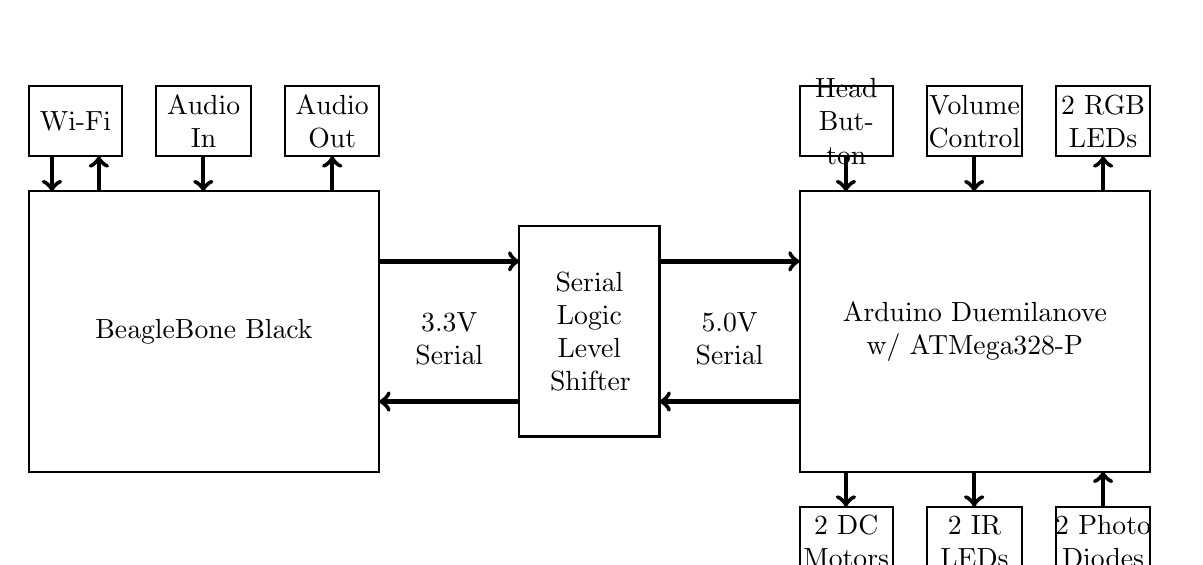
\begin{tikzpicture}[scale=0.89]
				\draw[thick](0, 4.5) rectangle node[]{Wi-Fi}(1.33, 5.5);
				\draw[ultra thick, <-] (0.33,4) -- (0.33, 4.5);
				\draw[ultra thick, ->] (1, 4) -- (1, 4.5);
				\draw[thick](1.82, 4.5) rectangle node[text width=1cm, align=center]{Audio In}(3.17, 5.5);
				\draw[ultra thick, <-] (2.49, 4) -- (2.49,4.5);
				\draw[thick](3.66, 4.5) rectangle node[text width=1cm, align=center]{Audio Out}(5, 5.5);
				\draw[ultra thick, ->] (4.33,4) -- (4.33,4.5);
				\draw[thick](0,0) rectangle node[]{BeagleBone Black}(5,4);
				\draw[ultra thick, <-] (5,1) -- (7,1);
				\draw[ultra thick, ->] (5,3) -- node[text width=1cm, align=center, below=0.5]{3.3V Serial}(7,3);
				\draw[thick](7,0.5) rectangle node[text width=1cm, align=center]{Serial Logic Level Shifter}(9,3.5);
				\draw[ultra thick, <-] (9,1) -- (11,1);
				\draw[ultra thick, ->] (9,3) -- node[text width=1cm, align=center, below=0.5]{5.0V Serial}(11,3);
				\draw[thick](11, 4.5) rectangle node[text width=1cm, align=center]{Head Button}(12.33, 5.5);
				\draw[ultra thick, <-] (11.66,4) -- (11.66,4.5);
				\draw[thick](12.82, 4.5) rectangle node[text width=1.2cm, align=center]{Volume Control}(14.17, 5.5);
				\draw[ultra thick, <-] (13.49,4) -- (13.49,4.5);
				\draw[thick](14.66, 4.5) rectangle node[text width=1.2cm, align=center]{2 RGB LEDs}(16, 5.5);
				\draw[ultra thick, ->] (15.33,4) -- (15.33,4.5);
				\draw[thick](11, 0) rectangle node[text width=3.6cm, align=center]{Arduino Duemilanove w/ ATMega328-P}(16,4);
				\draw[thick](11, -0.5) rectangle node[text width=1.2cm, align=center]{2 DC Motors}((12.33, -1.5);
				\draw[ultra thick, ->] (11.66,0) -- (11.66,-0.5);
				\draw[thick](12.82, -0.5) rectangle node[text width=1cm, align=center]{2 IR LEDs}((14.17, -1.5);
				\draw[ultra thick, ->] (13.49,0) -- (13.49,-0.5);
				\draw[thick](14.66, -0.5) rectangle node[text width=1.6cm, align=center]{2 Photo Diodes}((16, -1.5);
				\draw[ultra thick, <-] (15.33,0) -- (15.33,-0.5);
			\end{tikzpicture}
			}
			\caption[Initial overview of replacement hardware for Nabaztag:tag]{Initial high level overview of the replacement hardware for the Nabaztag:tag}
			\label{fig:initialhardware}
		\end{figure}
		
		\subsubsection{Custom AVR Board}
		
		To overcome the issues with using the full size Duemilanove board, it was decided to create a custom AVR board using the ATMega328-P microcontroller from the Duemilanove. The ATMega328-P can operate at lower voltages, and at 3.3V can sustain an 8MHz operating frequency using its internal oscillator, which will be sufficient for this project. This also means that the serial logic level will be 3.3V, so no logic level shifter is required. The revised architecture can be seen in \autoref{fig:revisedhardware}. 
		
		The microcontroller is removable, so can be programmed whilst on the Duemilanove board, using the \ac{USB} serial connection, before being removed and placed in the custom circuit for testing. Designing a custom board will enable all additional required components to be placed in a way that minimises the size of the board, meaning both the board and the \ac{BBB} will fit in the Nabaztag:tag.
		
		\begin{figure}[H]
			\centerline{
			\scriptsize
			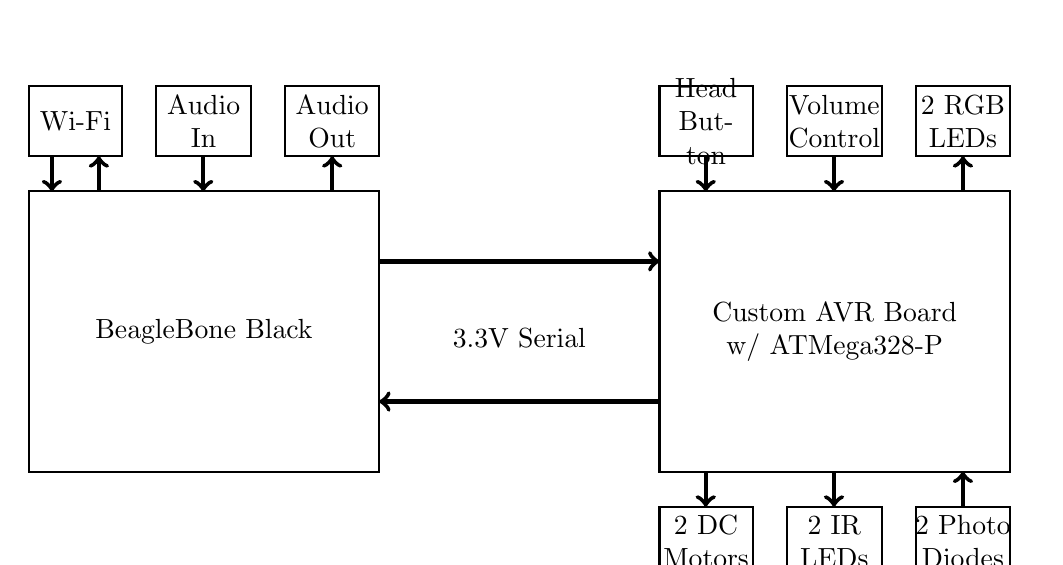
\begin{tikzpicture}[scale=0.89]
				\draw[thick](0, 4.5) rectangle node[]{Wi-Fi}(1.33, 5.5);
				\draw[ultra thick, <-] (0.33,4) -- (0.33, 4.5);
				\draw[ultra thick, ->] (1, 4) -- (1, 4.5);
				\draw[thick](1.82, 4.5) rectangle node[text width=1cm, align=center]{Audio In}(3.17, 5.5);
				\draw[ultra thick, <-] (2.49, 4) -- (2.49,4.5);
				\draw[thick](3.66, 4.5) rectangle node[text width=1cm, align=center]{Audio Out}(5, 5.5);
				\draw[ultra thick, ->] (4.33,4) -- (4.33,4.5);
				\draw[thick](0,0) rectangle node[]{BeagleBone Black}(5,4);
				\draw[ultra thick, <-] (5,1) -- (9,1);
				\draw[ultra thick, ->] (5,3) -- node[below=0.7]{3.3V Serial}(9,3);
				\draw[thick](9, 4.5) rectangle node[text width=1cm, align=center]{Head Button}(10.33, 5.5);
				\draw[ultra thick, <-] (9.66,4) -- (9.66,4.5);
				\draw[thick](10.82, 4.5) rectangle node[text width=1.2cm, align=center]{Volume Control}(12.17, 5.5);
				\draw[ultra thick, <-] (11.49,4) -- (11.49,4.5);
				\draw[thick](12.66, 4.5) rectangle node[text width=1.2cm, align=center]{2 RGB LEDs}(14, 5.5);
				\draw[ultra thick, ->] (13.33,4) -- (13.33,4.5);
				\draw[thick](9, 0) rectangle node[text width=3.6cm, align=center]{Custom AVR Board w/ ATMega328-P}(14,4);
				\draw[thick](9, -0.5) rectangle node[text width=1.2cm, align=center]{2 DC Motors}((10.33, -1.5);
				\draw[ultra thick, ->] (9.66,0) -- (9.66,-0.5);
				\draw[thick](10.82, -0.5) rectangle node[text width=1cm, align=center]{2 IR LEDs}((12.17, -1.5);
				\draw[ultra thick, ->] (11.49,0) -- (11.49,-0.5);
				\draw[thick](12.66, -0.5) rectangle node[text width=1.6cm, align=center]{2 Photo Diodes}((14, -1.5);
				\draw[ultra thick, <-] (13.33,0) -- (13.33,-0.5);
			\end{tikzpicture}
			}
			\caption[Revised overview of replacement hardware for Nabaztag:tag]{Revised high level overview of the replacement hardware for the Nabaztag:tag}
			\label{fig:revisedhardware}
		\end{figure}
		
		From this outline design, a schematic was created for the custom AVR board using Cadsoft's Eagle PCB Software \parencite{eaglepcb}. The original Arduino Duemilanove schematic \parencite{duemilanoveschematic} and the ATMega328-P pinout (\autoref{fig:atmegapinout} in Appendix \ref{app:atmegapinout}) were used for guidance. The schematic (\autoref{fig:avrschematicimage} in Appendix \ref{app:avrschematic}) integrates the additional circuitry required to control the ears, \acp{LED}, head button and volume control. A list of parts used in the schematic is available in \autoref{tab:partslist} in Appendix \ref{app:componentslist}.
		
		\subsection{Prototyping}
		
		Using the schematic as a guide, the various parts of the circuit were laid out on a breadboard (\autoref{fig:prototypeimage} in Appendix \ref{app:prototype}), and tested by connecting to the relevant female headers on the Nabaztag:tag hardware.
		
		In order to test the prototype, code was written for the ATMega328-P in the Arduino IDE, and flashed to the chip through the Duemilanove. Each section of the code was first tested using the relevant hardware from the Nabaztag:tag connected directly to the Arduino Duemilanove, and then retested with the ATMega328-P in the prototype board, and the relevant Nabaztag:tag hardware connected to the board.
		
		\autoref{fig:serialcommandcode} in Appendix \ref{app:exampleserial} shows a code example for serial communication with the ATMega328-P. It uses the SerialCommand library \parencite{serialcommand} to parse commands sent over the serial connection and call the relevant method, which then extracts arguments and performs the action. In the example given, sending \verb+EARPOS L+ would return the position of the left ear over the serial connection.
		
		\autoref{fig:isrcode} in Appendix \ref{app:exampleisr} shows a code example for an \ac{ISR} to handle moving the left ear. In this example, \verb+EARMOV+ is called using a serial command such as \verb+EARMOV L 10+, which will move the left ear to the tenth tooth on the encoder cog. When this command is issued, \verb+moveLeftEar+ is set as the \ac{ISR} for interrupt input one, and the ear is set in motion. Each time a tooth of the encoder cog breaks the \ac{IR} beam, an interrupt is triggered and \verb+moveLeftEar+ is called. It increments the variable storing the encoder tooth position, and stops the ear motor when the correct tooth, in this case 10, is reached. To enable a more logical control of ear position, the function translates a position of $0$ to the actual upright position of the ear, which is at encoder tooth 2.
		
	\subsection{Final Circuit}
	
	With prototyping showing the design was correct, the circuit was transferred to perfboard for installation in the Nabaztag:tag. The completed board is shown in \autoref{fig:avrboard}.
	
			\begin{figure}[H]
			\centerline{
				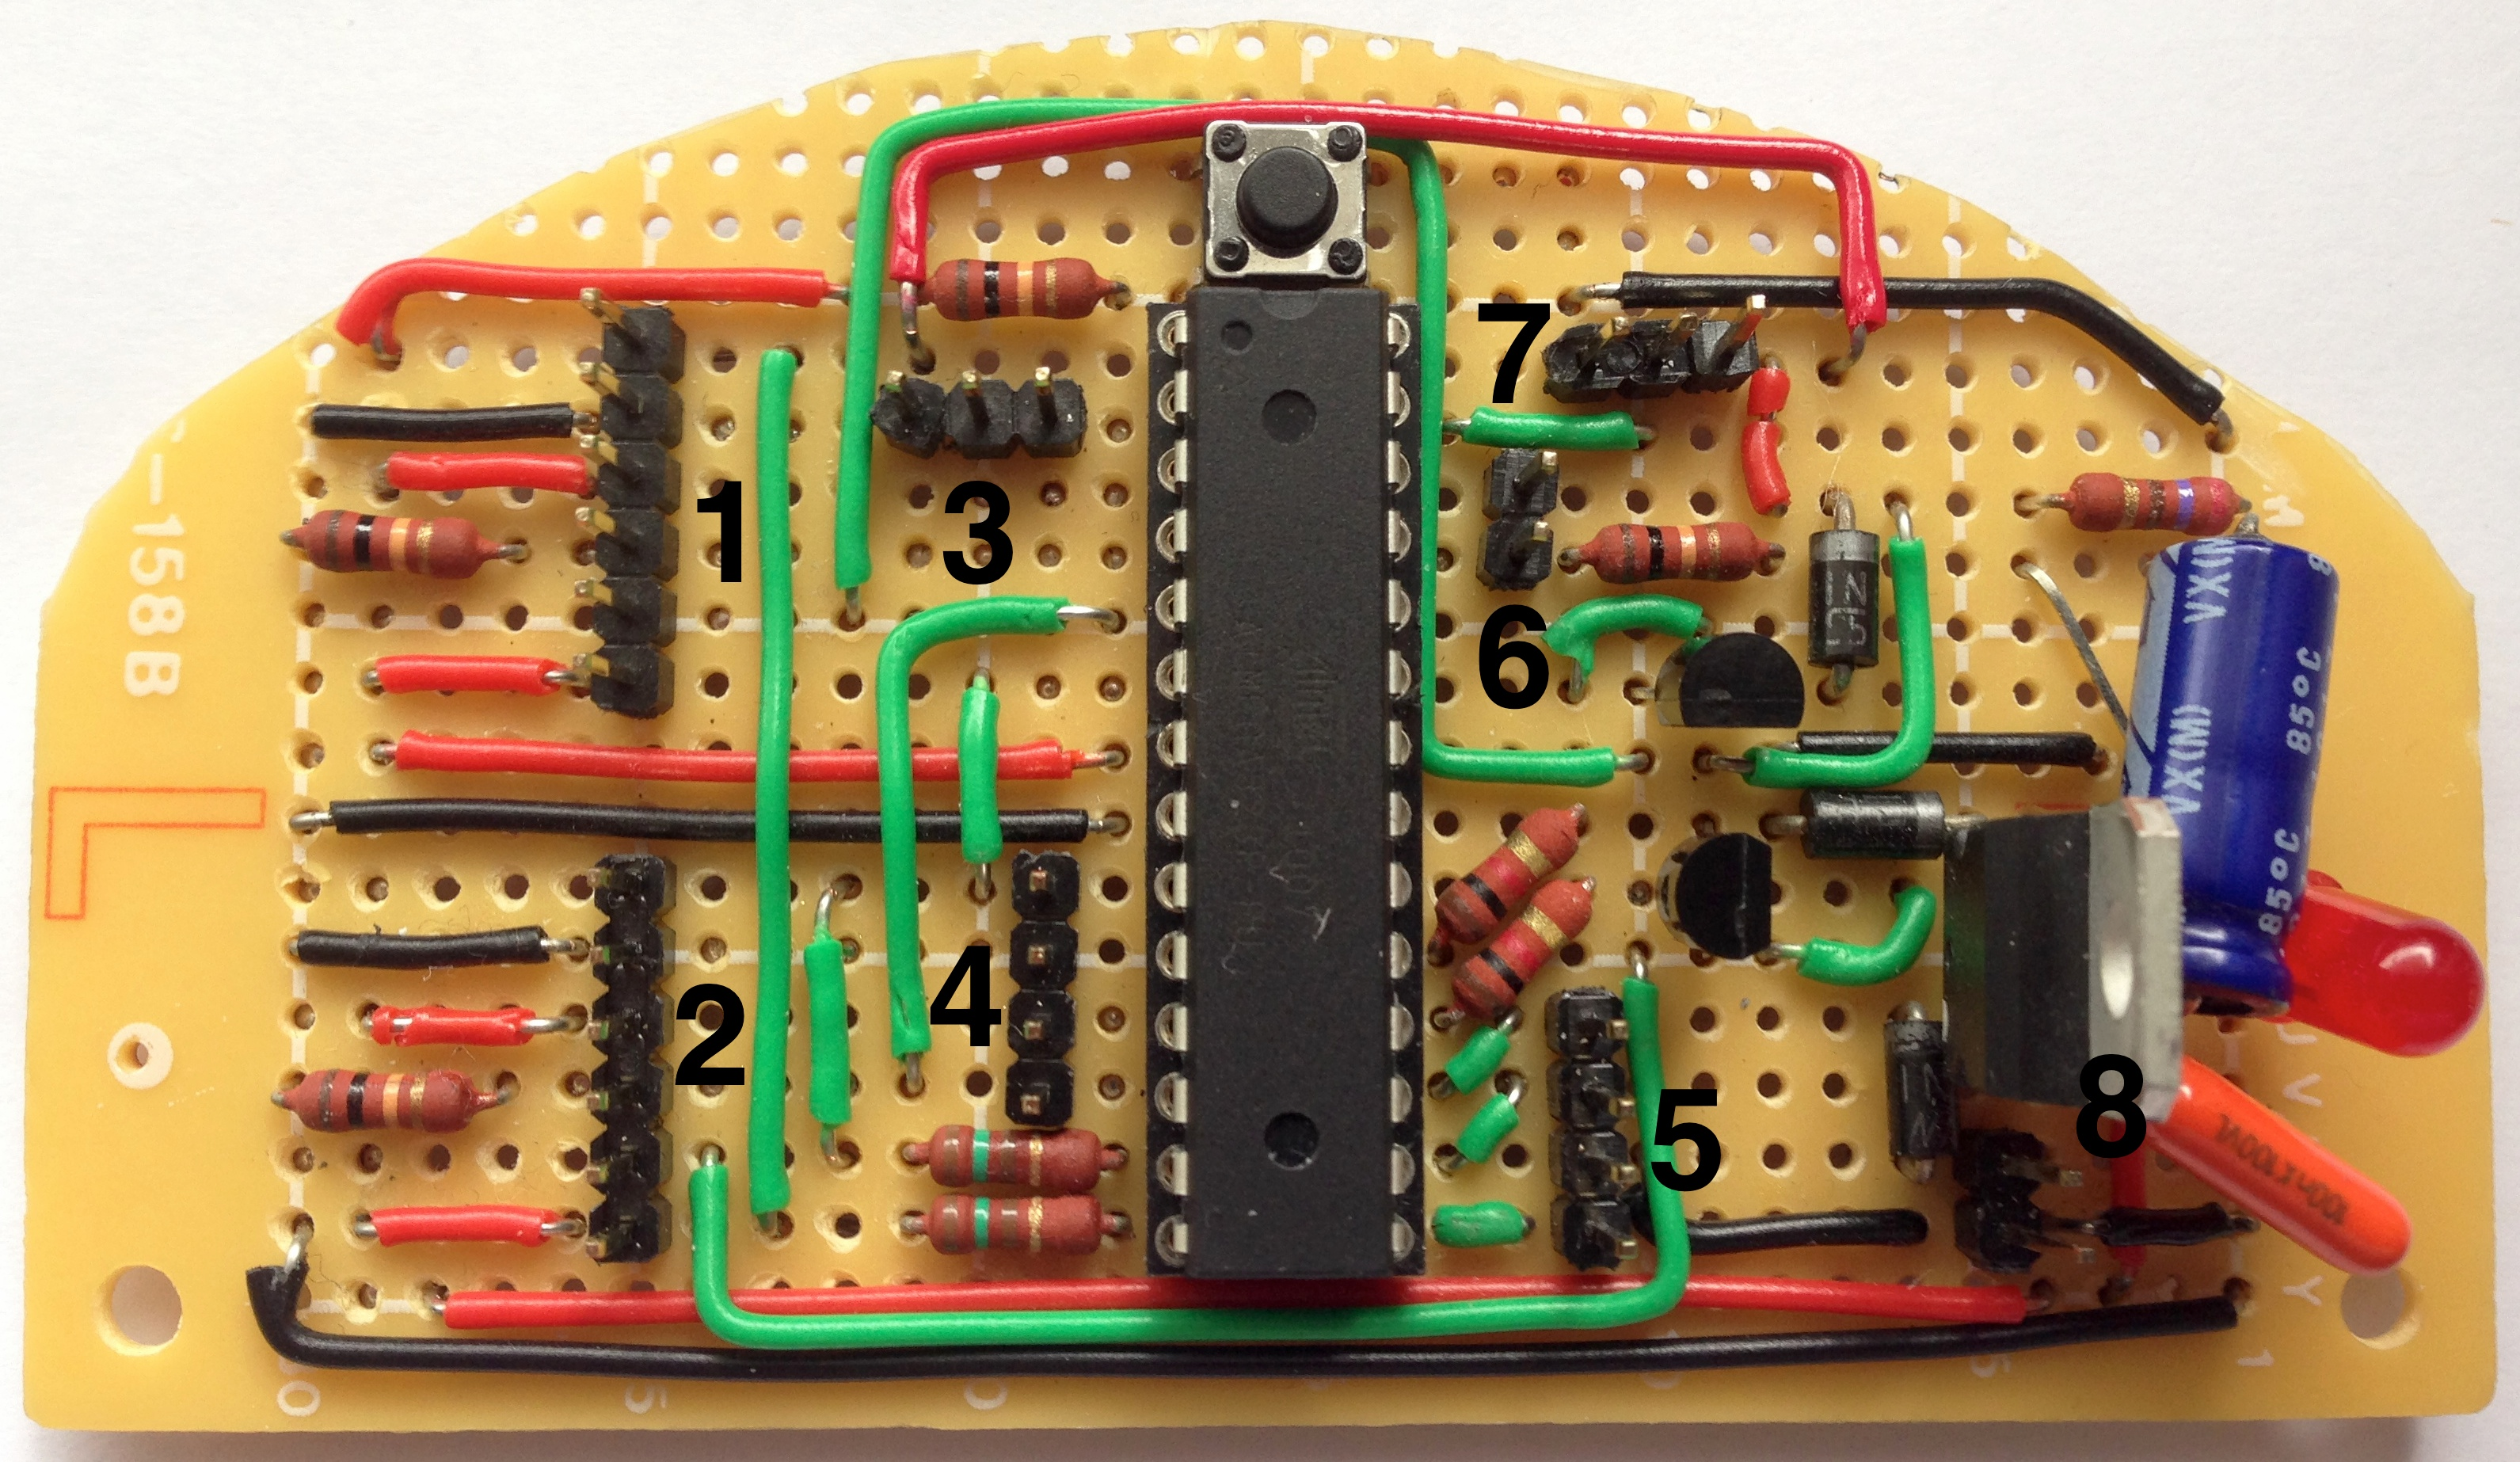
\includegraphics[scale=0.11]{images/avrboard.jpg}
			}
			\caption[Completed custom AVR board]{Completed custom AVR board. The headers are used as follows: 1) Right ear, 2) Left ear, 3) Serial connection to \ac{BBB}, 4) Bottom \ac{LED}, 5) Top \ac{LED}, 6) Head button, 7) Volume control - unused, 8) DC input.}
			\label{fig:avrboard}
		\end{figure}
		
	\subsection{Assembly}
	
	The final task after completion of the custom AVR circuit was to connect it with the \ac{BBB} and install them in the Nabaztag:tag shell. This also required finding a way to add audio functionality back to the Nabaztag:tag, and it was decided the simplest way to achieve this was to attach a \ac{USB} soundcard to the \ac{BBB}. This added an additional requirement of a small \ac{USB} hub as the \ac{BBB} has only a single \ac{USB} port, in use by the Wi-Fi adapter. Two different soundcards and two different small \ac{USB} hubs were ordered using the project budget to determine which would best fit in the Nabaztag:tag. Once these items were obtained, the assembly of the device was completed, as shown in Appendix \ref{app:assembled} in \autoref{fig:assembled1} and \autoref{fig:assembled2}. Although the circuit design included a header for the volume control, volume control functionality was not re-implemented.
		
	\section{Software}
	
	With the Nabaztag:tag re-assembled, attention moved to the software side of the project. A replacement software architecture was required to support both basic and more advanced functionality of the device.
	
	\subsection{Original Software Analysis}
	\label{sec:orig_analysis}
	
	Alongside the Nabaztag:tag hardware investigations used for reference earlier in the report, several projects have attempted to understand the software architecture which supported the Nabaztag ecosystem \parencite{Beausset2009, nabaztagxmpp1, nabaztagxmpp2, nabaztagxmpp3, nabaztagsoftwaredissection}. \citeauthor{Beausset2009} captured the traffic passing between a Nabaztag:tag and Violet's servers, identifying the protocol used to carry the messages as the \ac{XMPP} \parencite{Beausset2009}. \ac{XMPP} provides push, request-response, and publish-subscribe paradigms for message delivery, using \ac{XML} streams \parencite{Saint-Andre2005}. The technology was originally developed for Jabber, an open \ac{IM} service, whose core protocols were later standardised as \acs{XMPP} by the \ac{IETF} \parencite{rfc6120}.
	
	\begin{figure}[H]
	\centering
	\begin{subfigure}{0.95\textwidth}
	\begin{minted}[mathescape,linenos,numbersep=5pt,gobble=2, frame=lines,framesep=2mm]{xml}
		<iq from="net.violet.platform@xmpp.nabaztag.com/sources"
		to="0019db9ed017@xmpp.nabaztag.com/boot" id="3" type="result">
		  <query xmlns="violet:iq:sources">
		    <packet xmlns="violet:packet" format="1.0" ttl="604800">
		      fwQAAAx////+BAAFAA7/CAALAAABAP8=
		    </packet>
		  </query>
		</iq>
	\end{minted}
	\end{subfigure}
	\caption[A captured Nabaztag:tag XMPP message]{A captured \protect\ac{XMPP} message, sent from Violet's servers to a specific Nabaztag device (from \protect\parencite{Beausset2009}). The \protect\texttt{<iq />} stanza within the \protect\ac{XMPP} specification is a ``request-response mechanism, similar in many ways to HTTP, that lets entities make requests of and receive responses from each other'' \protect\parencite{Saint-Andre2005}}
	\label{fig:nabaztagxmpp}
	\end{figure}
	
	The \ac{XMPP} client software on the Nabaztag:tag ran entirely inside a purpose-made \ac{VM}, whose bootcode was retrieved from Violet's servers with an initial \ac{HTTP} request each time the Nabaztag:tag was turned on \parencite{nabaztagsoftwaredissection}. Once the \ac{VM} had booted, an authenticated \ac{XMPP} stream was established with Violet's servers, using the \ac{MAC} address of the Nabaztag:tag device as an identifier, and instructions for the device were sent over the stream as \verb+<iq />+ or \verb+<message />+ stanzas \parencite{nabaztagsoftwaredissection}.
	
	It is no longer possible to access the original Violet servers and there is no information available as to the specific reasons for the failing of the original architecture. A close approximation to the original architecture involved using an unaltered Nabaztag:tag with an open source server, Nabaztaglives \parencite{nabaztaglives}, but the experience was a frustrating one. Messages sent from the server often took a long period of time to reach the device, and were sometimes lost.
  
  It was decided that rather than attempting to recreate the \ac{XMPP} architecture, other technologies should be explored in the hope of achieving improved performance.
  			
\subsection{Requirements}

Based on the information from Section \ref{sec:nabaztaghist} and Section \ref{sec:orig_analysis}, a list of requirements for the software side of the project, shown in \autoref{tab:requirements}, was drawn up. The choices made to meet the requirements are addressed in Sections \ref{sec:require1} to Section \ref{sec:require7}

		\begin{center}
		\begin{longtable}{ | C{0.06\textwidth} | L{0.25\textwidth} | L{0.6\textwidth} |}
			\hline
			\textbf{No.} & \textbf{Requirement} & \textbf{Details} \\
			\hline
			\endfirsthead
			\multicolumn{3}{l}{\tablename\ \thetable\ --- \textit{Continued from previous page}} \\
			\hline \textbf{No.} & \textbf{Requirement} & \textbf{Details} \\ \hline
			\endhead
			\multicolumn{3}{r}{\textit{Continued on next page}} \\
			\endfoot
			\endlastfoot
			1 & A new communication protocol to replace \ac{XMPP}. & Due to the shortcomings of the previous infrastructure, where communication was performed over \ac{XMPP}, it was decided to explore a different technology for communication.\\
			\hline
			2 & A simple, consistent message format. & To help with development, and provide opportunities for expansion of functionality, a simple and  human readable message format with low overhead should be used.\\
			\hline
			3 & A web interface able to send control messages to the Nabaztag:tag. & For basic functionality, a simple web application should be created to control features of the Nabaztag:tag, e.g. control of the ears, \acp{LED} and \ac{TTS} functionality.\\
			\hline
			4 & Push communication of messages from server to Nabaztag:tag. & A major issue with Violet's infrastructure was the slow delivery of messages from the server to the device, a replacement system should attempt to solve this issue.\\
			\hline
			5 & Pairings should be possible between Nabaztag:tag devices. & To show more advanced functionality can be supported using the web application, pairings should be possible, where actions such as ear movements or button presses performed on one device are mirrored on any devices that are paired with it. This feature was advertised for the original Nabaztag:tag, but was very temperamental.\\
			\hline
			6 & The Nabaztag:tag should be location aware & The original Nabaztag:tag had no location awareness, so information such as weather was not available without the user configuring the location of the device.\\
			\hline
			7 & An advanced feature not seen before on the Nabaztag:tag should be implemented. & With a new open hardware and software system in place, a new feature should be implemented that would improve user interaction with the Nabaztag:tag and bring it more in line with current internet connected devices. \\
			\hline
		\caption{Requirements of replacement software architecture}
		\label{tab:requirements}
		\end{longtable}
	\end{center}

\subsubsection{Requirement 1}\label{sec:require1}
The initial requirement is to find a suitable alternative to \ac{XMPP}. We require full-duplex communication over a long-lived channel,  allowing messages to be sent from the server to the Nabaztag:tag, and vice versa, with minimal overhead. We look to \ac{HTTP} and its various mechanisms for achieving such communication.
	
WebSocket is a relatively young protocol, standardised by the \ac{IETF} in 2011 in \ac{RFC} 6455 \parencite{rfc6455}. It defines a bi-directional communication protocol over a single TCP connection. Whilst it was primarily designed for sending real-time data to web browsers, WebSocket clients can be implemented outside the browser in standalone applications.

Other methods do exist for creating long-lived connections over \ac{HTTP}, such as long-polling and \ac{XHR}-polling (often collectively referred to as Comet methods), but a number of papers have discussed the performance improvements of the newer WebSocket protocol over such methods.
		
\citeauthor{Gutwin2011} compared WebSockets to Comet methods in the context of browser-based collaborative applications, stating that ``real-time interaction has much stricter network requirements (in terms of update rate, message throughput, and latency) than semi-synchronous applications'' \parencite{Gutwin2011}. They found that round-trip latencies were between two and six times lower using WebSockets than with any of the Comet methods, with WebSockets showing the highest message per second throughput of any of the methods tested \parencite{Gutwin2011}. 
		
\citeauthor{Agarwal2012} showed that whilst \ac{XHR}-polling was limited to 44kbits/s, WebSockets were able to achieve a throughput of 66 kbits/s \parencite{Agarwal2012}. He found that ``XHR-polling imposes a large overhead of up to 5x'' because ``each interaction between a client and server is expressed in the form of HTTP requests and responses [...] for example, browser cookies and HTTP headers are included in each request and response'' \parencite{Agarwal2012}. By contrast he found only ``a 1.16x overhead in the case of HTML5 WebSockets'' (the baseline is the performance of a raw TCP socket) \parencite{Agarwal2012}.
	  
A third comparison was performed by \citeauthor{Puranik2013} in the context of a real-time monitoring system. They compared \ac{AJAX}, a technology making use of \ac{XHR}-polling, and WebSockets, finding that ``WebSockets can send up to 215.44\% more data samples when consuming the same amount of network bandwidth as \ac{AJAX}'' \parencite{Puranik2013}.

Given the results presented in these papers, it seems clear that the WebSocket protocol provides better performance than other long-lived \ac{HTTP} connection methods, and would be a suitable replacement for \ac{XMPP} in the Nabaztag:tag system.

\subsubsection{Requirement 2}
As highlighted in Section \ref{sec:orig_analysis}, the original Nabaztag:tag used \ac{XMPP}, meaning that messages were sent to and from the device in \ac{XML}. Whilst \ac{XML} is human-readable, parsing is expensive, requiring use of the \ac{DOM} \parencite{Lin2012}. \ac{JSON} \parencite{json} is a lightweight alternative to \ac{XML} introduced in 2001 \parencite{Severance2012}. \autoref{fig:xmlvjson} shows an example message in both \ac{XML} and \ac{JSON}.

	\begin{figure}[H]
		\centering
		\begin{subfigure}{0.27\textwidth}
		\centering
		\begin{minted}[fontfamily=tt,mathescape,linenos,numbersep=5pt,gobble=2,frame=single,framesep=2mm]{xml}
		<message>
		  <ear>L</ear>
		  <pos>10></pos>
		</message>
		\end{minted}
		\end{subfigure}
		~~~~~~~~~~~~~~~
		\begin{subfigure}{0.23\textwidth}
		\centering
		\begin{minted}[fontfamily=tt,mathescape,linenos,numbersep=5pt,gobble=2,frame=single,framesep=2mm]{json}
		{
		  "ear": "L",
		  "pos": 10
		}
		\end{minted}
		\end{subfigure}
		\caption[A comparison between \acs{XML} and \acs{JSON}]{A comparison between \ac{XML} (left) and \ac{JSON} (right)}
		\label{fig:xmlvjson}
	\end{figure}
	
	\vspace{-15pt}

In a comparison betwen \ac{XML} and \ac{JSON}, \citeauthor{Lin2012} found that for \ac{JSON} and \ac{XML} objects representing the same data, the \ac{JSON} object could be transmitted $30 - 35$\% faster, due to reduced redundancy in describing the data \parencite{Lin2012}. They also showed that, as the object size increases, the time taken to de-serialise \ac{JSON} remains reasonably constant, whilst the time taken to de-serialise the equivalent object in \ac{XML} increases significantly \parencite{Lin2012}.

\ac{JSON} will be used as a replacement for \ac{XML} in sending messages over the WebSocket connection between the server and the Nabaztag:tag.

\subsubsection{Requirements 3, 4 \& 5}
A web application meeting Requirement 3 will provide an easy to use interface for interacting with and managing Nabaztag:tag devices. The decision was made to use the Django Web Framework \parencite{django} as the author is familiar with the framework, having used it for a previous project. Django is written in Python, meaning the same programming language will be used for both client and server applications, aiding consistency in programming style.

In order to improve the quality of interactions with the Nabaztag:tag, it is important that messages sent to the device through the web application are seen to arrive instantaneously. Combined with Requirements 1 and 2, Requirement 4 identifies the need for a technology that is able to push messages in \ac{JSON} format from the server to a Nabaztag:tag connected via a WebSocket connection. \citeauthor{Brustel2012} describe push communication as being ``based on the general publish-and-subscribe model'' \parencite{Brustel2012}, in which a Subscriber subscribes to Topics offered by a Broker, and a Publisher publishes messages to the same topics. The diagram used in their explanation is reproduced in \autoref{fig:pubsubmodel}. In this example, a message for Topic B is published to the Broker, and any Subscribers subscribed to Topic B receive the message.

\begin{figure}[H]
	\centerline{
	\scriptsize
	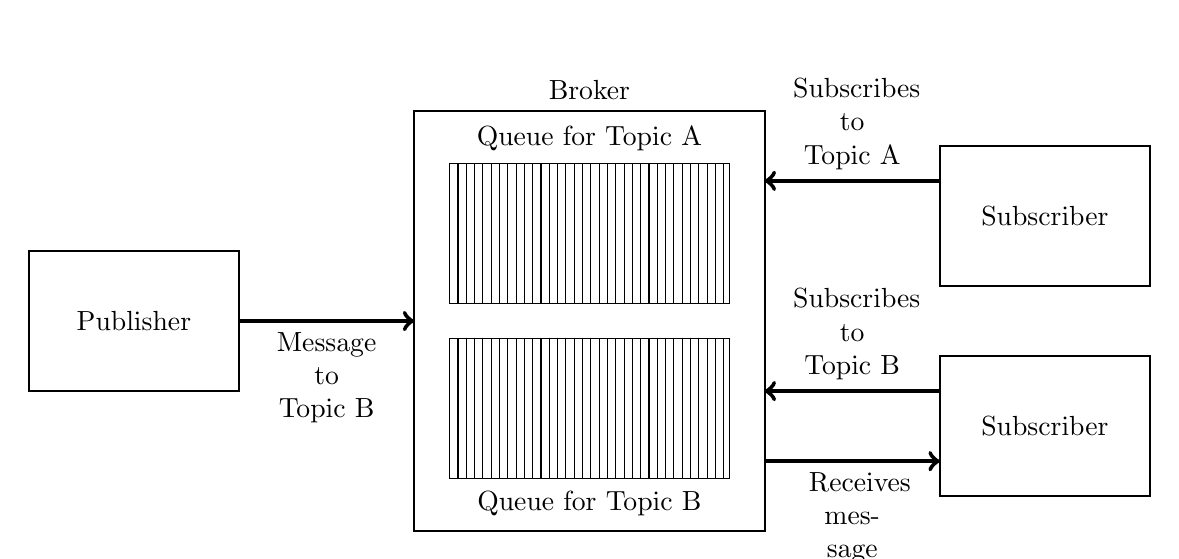
\begin{tikzpicture}[scale=0.89]
		\draw[thick] (0,2) rectangle node[align=center]{Publisher}(3,4);
		\draw[ultra thick, ->] (3,3) -- node[align=center, below, text width=1.5cm]{Message to Topic B}(5.5,3);
		\node[] at (8, 6.3) {Broker};
		\draw[thick] (5.5,0) rectangle (10.5, 6);
		\node[] at (8, 0.4) {Queue for Topic B};
		\draw[pattern=vertical lines, pattern color=black] (6,0.75) rectangle (10, 2.75);
		\node[] at (8, 5.6) {Queue for Topic A};
		\draw[pattern=vertical lines, pattern color=black] (6,3.25) rectangle (10, 5.25);
		\draw[ultra thick, <-] (10.5,5) -- node[align=center, above, text width=1.5cm]{Subscribes to Topic A}(13,5);
		\draw[thick] (13,3.5) rectangle node[align=center]{Subscriber}(16,5.5);
		\draw[ultra thick, <-] (10.5,2) -- node[align=center, above, text width=1.5cm]{Subscribes to Topic B}(13,2);
		\draw[thick] (13,0.5) rectangle node[align=center]{Subscriber}(16,2.5);
		\draw[ultra thick, ->] (10.5,1) -- node[align=center, text width=1.1cm, below]{Receives message}(13,1);
	\end{tikzpicture}
	}
	\caption[The publish-subscribe model]{The publish-subscribe model (reproduced from \protect\parencite{Brustel2012})}
	\label{fig:pubsubmodel}
\end{figure}

\vspace{-15pt}

With the decision to use Django to create the web application, a Django plugin, \ac{DWR} \parencite{djangowsredis}, was found that enables publish-subscribe behaviour over WebSocket connections. It uses Redis \parencite{redis}, a key-value store, to provide the message queues. A client connects to its own WebSocket using a unique identifier, and any messages placed by Django into a Redis queue with the same identifier are sent across the WebSocket to the client.

Requirement 5 can also be fulfilled as a consequence of using Django for the server application. Its use of the \ac{MVC} paradigm means that a class can be created to model a Nabaztag:tag, and separate instances of the class can be stored as pairs in a relation in Django's database.

\subsubsection{Requirement 6}
A general shortcoming of the Nabaztag:tag, identified by \citeauthor{Huang2011} \parencite{Huang2011}, was a lack of contextual awareness. An example of this was the device's weather information feature. As stated in \autoref{tab:origusecases} in Section \ref{sec:origusecases}, although the Nabaztag:tag did provide weather information, the user had to manually configure their location for this feature to work. \citeauthor{Abowd1999} define context as ``any information that can be used to characterise the situation of [...] a computational object'' \parencite{Abowd1999}, with the contextual information used to ``make its [the object's] behaviour more relevant to the situation in which it is being used'' \parencite{Abowd1999}.

With the advent of smartphones offering both Wi-Fi and \ac{GPS} technologies, companies such as Apple and Google have been able to collect large amounts of anonymised Wi-Fi base station addresses with associated \ac{GPS} co-ordinates. Google offers access to their version of this data using their GeoLocation API \parencite{googlegeo}. Using the Wi-Fi capabilities of the new Nabaztag:tag hardware, we can automatically obtain a reasonably accurate estimation of the Nabaztag:tag's current location, removing a user configuration step and improving the contextual awareness of the device.

\subsubsection{Requirement 7}\label{sec:require7}
The final requirement is open-ended, we must add a feature to the Nabaztag:tag that was previously not possible, but that adds some utility or function. The major shortcoming of the Nabaztag:tag was its complete reliance on Violet's supporting infrastructure. The eventual failure of this infrastructure resulted in thousands of owners with useless Nabztag:tag devices, and drove the more technically minded to the projects mentioned in Section \ref{sec:nabaztaghist} in attempts to bring their devices back to life.

A truly useful feature, then, would be to enable direct communication with the Nabaztag:tag, removing the central point of failure, and allowing infinitely more customisable interactions with the device. The concept of the \ac{IoT} was introduced in Section \ref{sec:litreview}, and to meet Requirement 7 we turn to a specific embodiment of this idea termed the \ac{WoT}, which is simply the \ac{IoT} concept applied specifically to the Web and Web technologies. \citeauthor{Gupta2011} define the \ac{WoT} as ``everyday objects [...] seamlessly integrated into the World Wide Web (WWW) using its well-known standards and blueprints, e.g. URIs, HTTP and REST.'' \parencite{Gupta2011}.

\ac{REST} is an architectural style for the Web introduced by Roy \citeauthor{Fielding2000} in his Doctoral Thesis \parencite{Fielding2000}. \citeauthor{Guinard2011} offered that ``the essence of REST is to focus on creating loosely coupled services on the Web, so that they can be easily reused.'' \parencite{Guinard2011}. Following the principles of \ac{REST}, the aim is to allow the resources of the Nabaztag:tag to be easily accessed and used by its owners.

To fulfil this requirement, the Nabaztag:tag's resources, e.g. ears, \acp{LED}, location awareness, and \ac{TTS} will be made available via an \ac{API} residing on the device. It will make use of two of \ac{HTTP}'s four main methods to interact with resources --- \verb+GET+ and \verb+PUT+. This will enable easy use of the resources, and enable third party applications to be created with full access to the Nabaztag:tag's features. Although there are Django plugins available for creating \ac{REST}ful \acp{API}, Django is unnecessarily heavyweight for a simple \ac{API} such as this, especially as it will be running on the \ac{BBB}. Flask \parencite{flask} is a lightweight web framework, enabling quick creation of \ac{REST}ful \acp{API}, and the Flask-\ac{REST}ful plugin \parencite{flaskrestful} adds support for class-based creation of \acp{API}. Again the framework is written in Python, which benefits development and code consistency.

	\subsection{Design}

	With the requirements of the system outlined, and major choices of frameworks and libraries made, we move on to the design of the system.	
	
	\subsubsection{System Architecture}
	
	\begin{figure}[H]
		\centerline{
		\scriptsize
		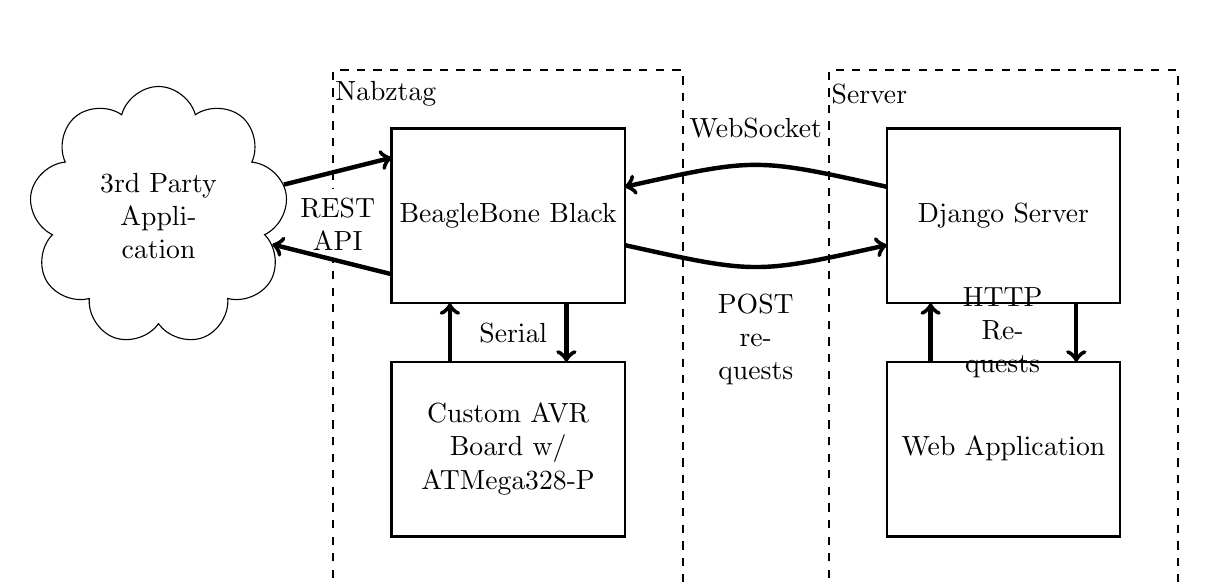
\begin{tikzpicture}[scale=0.74]
			% Nabaztag
			\node[] at (0.9,8.6) {Nabztag};
			\draw[thick, dashed](0,0) rectangle (6,9);
			\draw[thick](1,5) rectangle node{BeagleBone Black}(5,8);	
			\draw[ultra thick, ->] (2,4) -- node[right=0.23]{Serial}(2,5);
			\draw[ultra thick, <-] (4,4) -- (4,5);
			\draw[thick](1,1) rectangle node[text width=2.5cm, align=center]{Custom AVR Board w/ ATMega328-P}(5,4);
			\draw[ultra thick, <-] (5,7) .. controls (7.25,7.5) .. node[align=center, above=0.2]{WebSocket}(9.5,7);
			\draw[ultra thick, ->] (5,6) .. controls (7.25,5.5) .. node[align=center, text width=1.2cm, below=0.2]{POST requests}(9.5,6);
			% Server
			\node[] at (9.2,8.6) {Server};
			\draw[thick, dashed](8.5,0) rectangle (14.5,9);
			\draw[thick](9.5,5) rectangle node{Django Server}(13.5,8);
			\draw[ultra thick, ->] (10.25,4) -- node[text width=1.2cm, right=0.17, align=center]{HTTP Requests}(10.25,5);
			\draw[ultra thick, <-] (12.75,4) -- (12.75,5);
			\draw[thick](9.5,1) rectangle node{Web Application}(13.5,4);
			\node[draw, cloud, cloud puffs=9, text width=1.7cm, align=center] at (-3, 6.5) (cloud) {3rd Party Application};
			\draw[ultra thick, ->] (cloud) -- node[below=0.2, text width=1cm, align=center, fill=white]{REST API}(1, 7.5);
			\draw[ultra thick, <-] (cloud) -- (1, 5.5);
		\end{tikzpicture}
		}
		\caption[Overview of system architecture for Nabaztag:tag]{High level overview of the proposed system architecture for the Nabaztag:tag}
		\label{fig:systemarch}
	\end{figure}	
	
	
	Using the choices identified in Sections \ref{sec:require1} to \ref{sec:require7} a high level architecture is proposed for the system in \autoref{fig:systemarch}. In this design, a bi-directional WebSocket connection is established between a client running on the \ac{BBB} in the Nabaztag:tag, and a Django server instance running the \ac{DWR} plugin. The user of the Nabaztag:tag can interact with the device through a web application, their actions in the application are sent to the Django server as \ac{HTTP} requests, then transformed to corresponding \ac{JSON} messages for transmission over the WebSocket. The \ac{BBB} converts the \ac{JSON} message to a serial string suitable for the SerialCommand library running on the ATMega328-P AVR.
	
	For events occurring on the Nabaztag:tag, such as the user moving the ears or pressing the head button, a \ac{JSON} message is created on the AVR, sent to the \ac{BBB} via the serial connection, and then forwarded on to the Django server using a \ac{HTTP} \verb+POST+ request for processing. In this case the Django application will determine if any Nabaztag:tags are paired with the sender of the message, and update them accordingly. Although ideally the design would fully utilise the bi-directional nature of the WebSocket in order to send updates to the server, the \ac{DWR} library chosen doesn't currently support this behaviour, only allowing messages placed into the WebSocket by the client to be stored in Redis, and not allowing them to trigger actions in the Django event loop \parencite{djangowsredis}. This library is under active development, so this feature may be available in the future.
	
	Finally, a \ac{REST}ful \ac{API} also runs on the \ac{BBB}. \ac{HTTP} requests to the \ac{API} endpoints are transformed to serial strings suitable for the SerialCommand library running on the ATMega328-P AVR.
	
	\subsubsection{Django Application}
	
	The Django application is relatively simple, the database stores information for each registered Nabaztag:tag device, and its structure is created from the model classes shown in \autoref{fig:djangoclassdiagram} using Django's \verb+syncdb+ tool. Each Nabaztag:tag device is represented within the application by a \verb+Nabaztag+ class instance, and a pairing between registered Nabaztag:tags by a \verb+PairedNabaztags+ class instance.
		
	\begin{figure}[H]
	\centering
	\scriptsize
		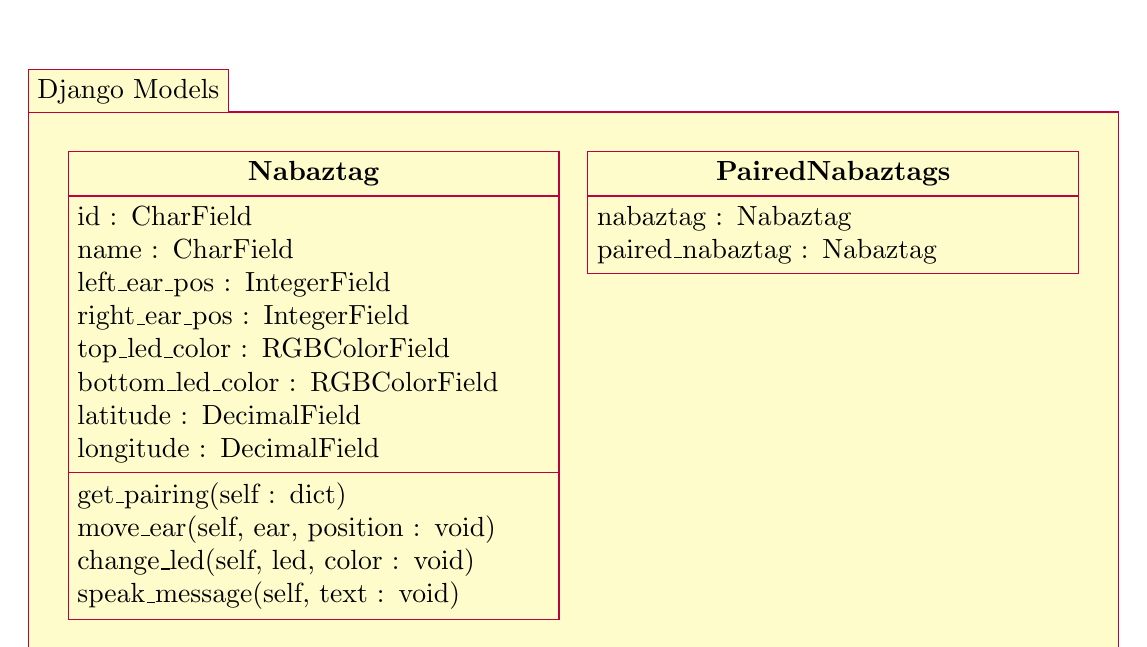
\begin{tikzpicture}
		\begin{package}{Django Models}
		  \begin{class}[text width=6cm]{Nabaztag}{0,0}
		    \attribute{id : CharField}
		    \attribute{name : CharField}
		    \attribute{left\_ear\_pos : IntegerField}
		    \attribute{right\_ear\_pos : IntegerField}
		    \attribute{top\_led\_color : RGBColorField}
		    \attribute{bottom\_led\_color : RGBColorField}
		    \attribute{latitude : DecimalField}
		    \attribute{longitude : DecimalField}
		    \operation{get\_pairing(self : dict)}
		    \operation{move\_ear(self, ear, position : void)}
		    \operation{change\_led(self, led, color : void)}
		    \operation{speak\_message(self, text : void)}
		  \end{class}
		
		  \begin{class}[text width=6cm]{PairedNabaztags}{6.6,0}
		    \attribute{nabaztag : Nabaztag}
		    \attribute{paired\_nabaztag : Nabaztag}
		  \end{class}
		\end{package}
		\end{tikzpicture}
	\caption[Class diagram for Django model classes]{Class diagram for Django model classes, showing the properties and methods of a \texttt{Nabaztag} object, and the pairing relationship between two Nabaztags.}
	\label{fig:djangoclassdiagram}
	\end{figure}
	
	\vspace{-15pt}
	
	It was decided to continue to use the \ac{MAC} address of a Nabaztag:tag as its identifier when registering it with the Django application.
	
	Webpages in the application are handled by defined view classes with associated templates that are instantiated when a particular \ac{URL} pattern is matched. Visiting the root of the site displays an index page where a list of registered Nabaztag:tags is displayed.

	Selecting a Nabaztag:tag takes the user to a page, shown in Appendix \ref{app:djangoapp} in \autoref{fig:djangoapp}, where they can view information about the device and control it. There are a variety of forms controlling different functions of the device. When a form is submitted, the appropriate notification method in the \verb+Nabaztag+ class instance is called, e.g. \verb+move_ear+, \verb+change_led+ or \verb+speak_message+, which converts the command to a \ac{JSON} message and places it in the Redis queue identified by the ID of the Nabaztag:tag. If a Nabaztag:tag client is connected via a WebSocket with a matching ID, it will receive the message.
	
	In order to handle updates via \verb+POST+ requests from Nabaztag:tag devices, an \ac{API} was created using the Django \ac{REST} Framework plugin \parencite{djangorest}. This plugin provides class-based \ac{API} creation, where the developer creates methods, such as \verb+post+ and \verb+get+ that they wish to provide functionality for. Three \verb+POST+ methods are provided by the \ac{API}:
	
	\begin{itemize}
		\item \verb+/update/<id>/ear+ - If an ear was moved on the device.
		\item \verb+/update/<id>/button+ - If the head button was pressed on the device
		\item \verb+/update/<id>/location+ - To allow the device to update its current location.
	\end{itemize}
	

	\subsubsection{Nabaztag:tag Client}
	
	Creating the web application was fairly simple as Django handles much of the heavy lifting, however there was no similar framework available to help develop the client application, the classes of which are shown in \autoref{fig:wsclassdiagram}.
	
	\begin{figure}[H]
	\centerline{
	\scriptsize
		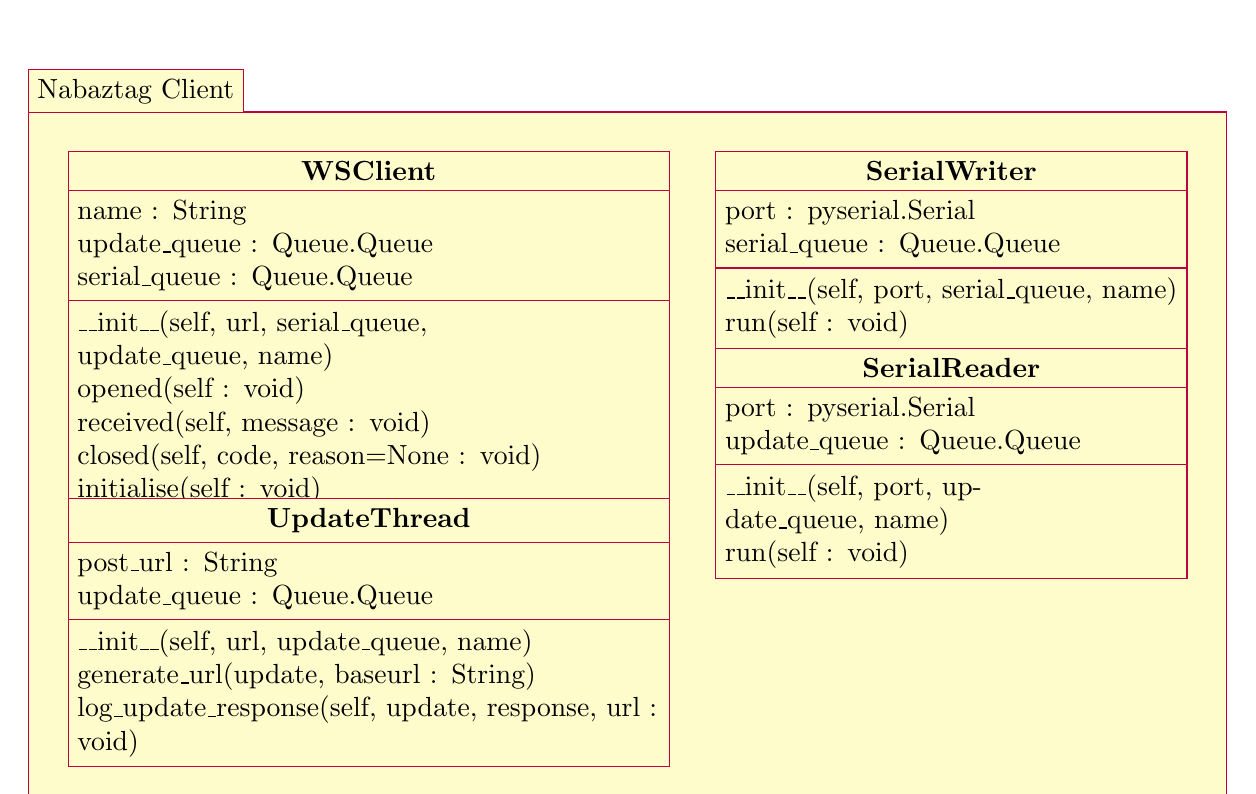
\begin{tikzpicture}
		\begin{package}{Nabaztag Client}
		  \begin{class}[text width=7.4cm]{WSClient}{0,0}
		  	\attribute{name : String}
		    \attribute{update\_queue : Queue.Queue}
		    \attribute{serial\_queue : Queue.Queue}
		    \operation{\_\_init\_\_(self, url, serial\_queue, update\_queue, name)}
		    \operation{opened(self : void)}
		    \operation{received(self, message : void)}
		    \operation{closed(self, code, reason=None : void)}
		    \operation{initialise(self : void)}
		    \operation{update\_server\_location(self : void)}
		    \operation{json\_to\_serial(json\_message : String)}
		  \end{class}
		  \begin{class}[text width=7.4cm]{UpdateThread}{0,-4.4}
		  	\attribute{post\_url : String}
		  	\attribute{update\_queue : Queue.Queue}
		  	\operation{\_\_init\_\_(self, url, update\_queue, name)}
		    \operation{generate\_url(update, baseurl : String)}
		    \operation{log\_update\_response(self, update, response, url : void)}
		  \end{class}
		  \begin{class}[text width=5.75cm]{SerialWriter}{7.4,0}
		  	\attribute{port : pyserial.Serial}
		    \attribute{serial\_queue : Queue.Queue}
		   	\operation{\_\_init\_\_(self, port, serial\_queue, name)}
		    \operation{run(self : void)}
		  \end{class}
		  \begin{class}[text width=5.75cm]{SerialReader}{7.4,-2.5}
		  	\attribute{port : pyserial.Serial}
		    \attribute{update\_queue : Queue.Queue}
		   	\operation{\_\_init\_\_(self, port, update\_queue, name)}
		    \operation{run(self : void)}
		  \end{class}
		\end{package}
		\end{tikzpicture}
	}
	\caption[Class diagram for the Nabaztag client application]{Class diagram for the Nabaztag client application. Shows the use of callback methods in the \texttt{WSClient} class, and shows use of threads and queues in other parts of the application}
	\label{fig:wsclassdiagram}
	\end{figure}
		
	Two key communication protocols had to be incorporated into the application. Serial communication with the \ac{BBB} is provided by the \verb+pyserial+ library \parencite{pyserial}, whilst WebSocket communication with the Django application is provided by the \verb+ws4py+ library \parencite{ws4py}. This was found to be the simplest WebSocket library to work with, allowing inheritance from a threaded \verb+WebSocketClient+ class and simply requiring the developer to override the necessary callback methods such as \verb+opened()+, \verb+received_message()+ and \verb+closed()+. These methods are then performed upon successful opening of the WebSocket connection, upon receipt of each message, and upon an expected (or unexpected) termination of the connection respectively. Other WebSocket libraries available either had more dependencies or required that callbacks be registered when initialising the class, making for more complex code.

The methods provided by \verb+pyserial+ for reading from and writing to the serial port are blocking, so it was decided to perform serial reads and writes in separate threads, both distinct from the WebSocket thread. Using Python's core \verb+Queue+ library, two queues were created to achieve communication between the separate threads. One queue handles messages arriving from the server over the WebSocket connection, and the other handles messages arriving from the AVR over the serial connection. The library provides the necessary locking to ensure the queues are thread safe.

A \verb+WSClient+ instance receives \ac{JSON} messages, e.g. \verb+{"ear": "L", "pos": 10}+, from the server and converts them to serial messages, e.g. \verb+EARMOV L 10+, before placing them in the \verb+serial_queue+ queue. This is monitored by a \verb+SerialWriter+ instance, and messages are taken from the queue and written to the serial port, to be received by the AVR.

 A \verb+SerialReader+ instance receives \ac{JSON} messages from the AVR and places them in the \verb+update_queue+ queue. This is monitored by an \verb+UpdateThread+ instance, which takes messages from the queue and sends \verb+POST+ requests containing the message to the correct \ac{API} method in the Django application.
 
	\subsubsection{\acs{REST}ful \acs{API}}
	
	The use of Flask with the Flask-Restful plug-in allowed the \ac{API} to be created quickly using knowledge learnt from developing the two previous parts of the system. Here the \verb+pyserial+ library is still required to send messages to the AVR, but a WebSocket connection is no longer required, so \verb+ws4py+ is not used.
	
	Similar to the approach used in the Django \ac{REST} Framework, an \ac{API} resource is created by inheriting from a \verb+Resource+ class and overriding the methods which should be made available as \ac{API} endpoints. \autoref{fig:apiclassdiagram} shows the five endpoints provided by the Nabaztag:tag \ac{API} and the \ac{HTTP} methods available for each. The parameters of the methods, e.g. \verb+ear+ in \verb+NabaztagEar+'s \verb+put(self, ear)+ method are defined in the \ac{URL} for the resource, e.g \verb+/nabaztag/api/ear/<string:ear>+, so a PUT request made to \verb+/nabaztag/api/ear/left+ would call the \verb+put+ method of the \verb+NabaztagEar+ class, with \verb+ear="left"+. All requests to and responses from the \ac{API} are in \ac{JSON} format.
	
	By specifying an instance of the \verb+RequestParser+ class for each method to parse the body of a received request, Flask-Restful can handle many common errors automatically. It can detect if parameters are of the wrong type or are not present, and return an error to the user of the \ac{API}. Other checks were manually implemented, such as ensuring ear position values and colour values were within allowed ranges.
	
	\begin{figure}[H]
	\centerline{
	\scriptsize
		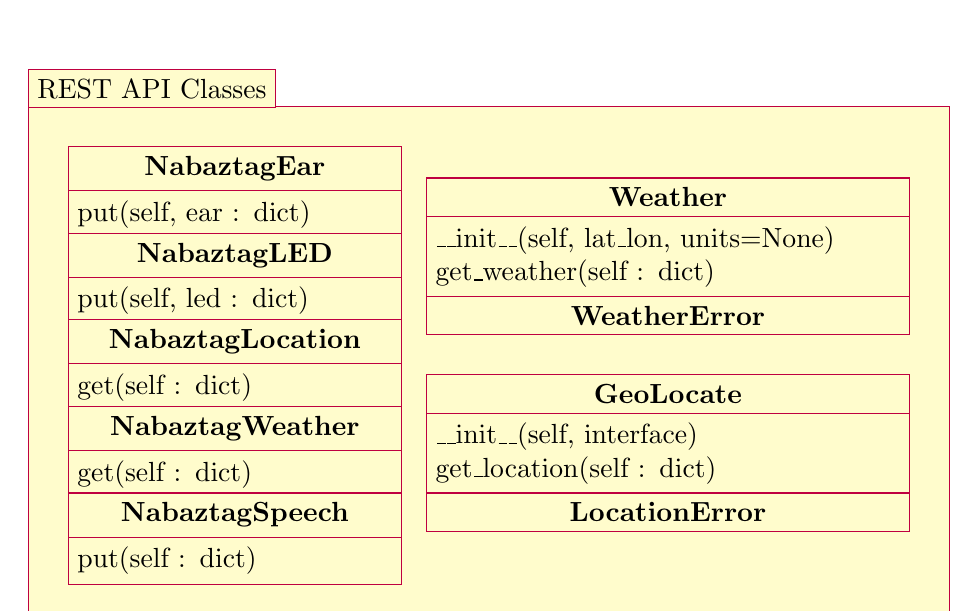
\begin{tikzpicture}
		\begin{package}{REST API Classes}
		  \begin{class}[text width=4cm]{NabaztagEar}{0,4.4}
		  	\operation{put(self, ear : dict)}
		  \end{class}
		  \begin{class}[text width=4cm]{NabaztagLED}{0,3.3}
		  	\operation{put(self, led : dict)}
		  \end{class}
		  \begin{class}[text width=4cm]{NabaztagLocation}{0,2.2}
		  	\operation{get(self : dict)}
		  \end{class}
		  \begin{class}[text width=4cm]{NabaztagWeather}{0,1.1}
		  	\operation{get(self : dict)}
		  \end{class}
		  \begin{class}[text width=4cm]{NabaztagSpeech}{0,0}
		  	\operation{put(self : dict)}
		  \end{class}
		  \begin{class}[text width=5.9cm]{Weather}{5.5,4}
		  	\operation{\_\_init\_\_(self, lat\_lon, units=None)}
		  	\operation{get\_weather(self : dict)}
		  \end{class}
		  \begin{class}[text width=5.9cm]{WeatherError}{5.5,2.5}
		  \end{class}
		  \begin{class}[text width=5.9cm]{GeoLocate}{5.5,1.5}
		  	\operation{\_\_init\_\_(self, interface)}
		  	\operation{get\_location(self : dict)}
		  \end{class}
		  \begin{class}[text width=5.9cm]{LocationError}{5.5,0}
		  \end{class}
		\end{package}
		\end{tikzpicture}
	}
	\caption[Class diagram for the \acs{REST}ful \acs{API}]{Class diagram for the Nabaztag:tag \ac{REST}ful \ac{API}}
	\label{fig:apiclassdiagram}
	\end{figure}
	
The \verb+Weather+ and \verb+GeoLocate+ classes interact with the OpenWeatherMap \ac{API} \parencite{openweather} and Google's GeoLocate \ac{API} \parencite{googlegeo} respectively, parsing the results and making them available through the Nabaztag:tag's \ac{API}. In case either third party service returns an error, custom Python errors \verb+WeatherError+ or \verb+LocationError+ are raised so that the \ac{API} can act accordingly.
	
During development of the \ac{API}, a markdown-based language called \ac{API} Blueprint \parencite{apiblueprint} was used to describe its structure. This enabled full documentation, in the form of a static webpage, to be created easily using a tool called Aglio \parencite{aglio}. This documentation was made available directly from the Nabaztag:tag device, from the root of the \ac{API}, so Nabaztag:tag users can access the documentation from a \ac{URL} following a similar pattern to the \ac{API} itself. An example section of this documentation for the NabaztagEar \ac{API} method is shown in Appendix \ref{app:apidoc} in \autoref{fig:apidoc}.
	
	\subsection{Deployment}
	
	Deployment of the system is treated separately for each application, as each requires a different configuration.
	
	\subsubsection{Django Application}
	
	Following the deployment instructions given in the documentation for the \ac{DWR} plugin \parencite{djangowsredis}, the most scalable deployment solution was chosen, with the structure shown in \autoref{fig:djangodeployment}. An open-source \ac{HTTP} server, Nginx \parencite{nginx}, is used as a front-end proxy server. Nginx version 1.4 introduced support for proxying WebSocket connections. \ac{WSGI} is a specification for interfacing between Python applications and web servers, and uWSGI \parencite{uwsgi} is a popular implementation of this, encapsulating applications like Django and allowing \ac{HTTP} servers to talk to them using \ac{WSGI}.
	
		\begin{figure}[H]
		\centerline{
		\footnotesize
		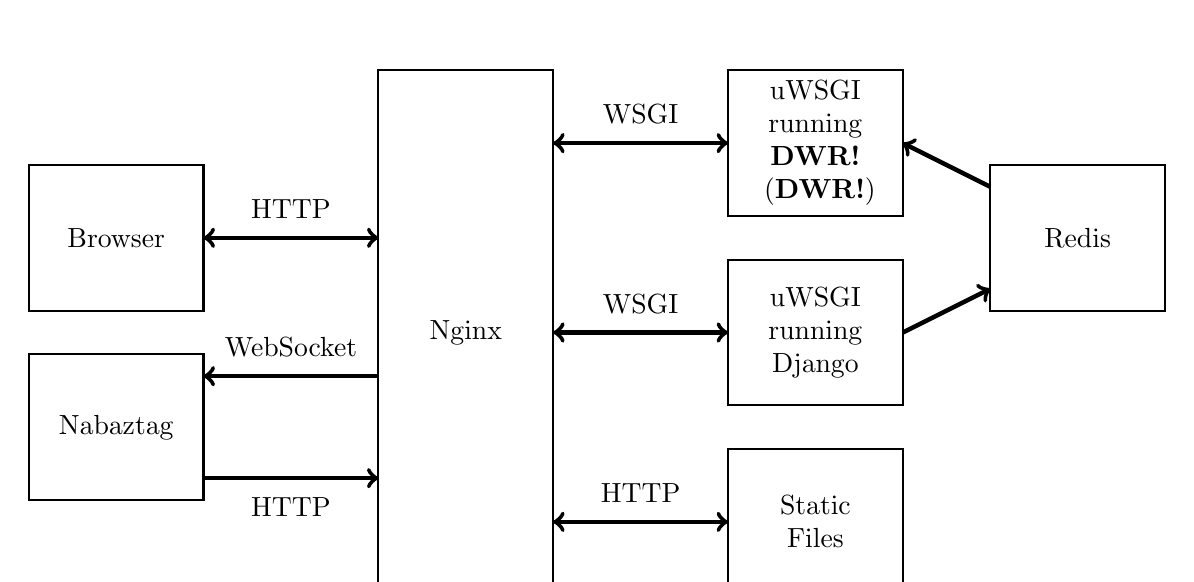
\begin{tikzpicture}[scale=0.74]
			%Browser
			\draw[thick](-0.5,4.875) rectangle node[]{Browser}(2.5,7.375);
			\draw[ultra thick, <->] (2.5,6.125) -- node[align=center, above=0.1]{HTTP}(5.5,6.125);		
			% Nabaz
			\draw[thick](-0.5,1.625) rectangle node[]{Nabaztag}(2.5,4.125);
			\draw[ultra thick, <-] (2.5,3.75) -- node[align=center, above=0.1]{WebSocket}(5.5,3.75);
			\draw[ultra thick, ->] (2.5,2) -- node[align=center, below=0.1]{HTTP}(5.5,2);
			% Nginx
			\draw[thick](5.5,0) rectangle node[]{Nginx}(8.5,9);
			\draw[ultra thick, <->] (8.5,7.75) -- node[align=center, above=0.1]{WSGI}(11.5,7.75);
			\draw[ultra thick, <->] (8.5,4.5) -- node[align=center, above=0.1]{WSGI}(11.5,4.5);
			\draw[ultra thick, <->] (8.5,1.25) -- node[align=center, above=0.1]{HTTP}(11.5,1.25);
			% uWSGI
			\draw[thick](11.5,6.5) rectangle node[align=center, text width=1.3cm]{uWSGI running \ac{DWR}}(14.5, 9);
			\draw[thick](11.5,3.25) rectangle node[align=center, text width=1.3cm]{uWSGI running Django}(14.5,5.75);
			\draw[thick](11.5,0) rectangle node[align=center, text width=1cm]{Static Files}(14.5,2.5);
			% Redis
			\draw[thick](16,4.875) rectangle node[]{Redis}(19,7.375);
			\draw[ultra thick, <-] (14.5,7.75) -- (16,7);
			\draw[ultra thick, ->] (14.5,4.5) -- (16,5.25);
		\end{tikzpicture}
		}
		\caption[Deployment diagram for Django application]{Deployment diagram for Django application (adapted from \parencite{djangowsredis})}
		\label{fig:djangodeployment}
	\end{figure}
	
	The configuration works as follows:	
	
	\begin{itemize}
		\item Static files needed for the Django application, such as stylesheet and image files, are served directly by Nginx.
		\item A \ac{URL} path of \verb+/ws/+ is defined in the Nginx configuration, and requests to \acp{URL} matching this are proxied by Nginx to a uWSGI instance running the \ac{DWR} plugin.
		\item All other requests, which are for pages generated by Django, are proxied by Nginx to a uWSGI instance running the Django application.
		\item The Django application communicates with the \ac{DWR} plugin solely through Redis message queues.
	\end{itemize}
	
	uWSGI provides a tool called \verb+emperor+, which can monitor a directory for configuration files, and start a separate uWSGI instance for each one. The \verb+emperor+ tool is configured to run on startup using Ubuntu's \verb+upstart+ utility, and configuration files for the Django and \ac{DWR} uWSGI instances are placed in the directory it monitors, ensuring they are run on startup. All configuration files and a readme for this deployment are available in the submitted archive, in the \verb+nabaztagserver/deployment+ directory.
	
	\subsubsection{Nabaztag:tag Client}
	
	The client application is also deployed using the \verb+upstart+ utility, which registers it as a system service, allowing it to be started and stopped by the user. It is automatically started on boot, reading its configuration information from a file.
	
	\ac{TTS} is provided by Festival \parencite{festival}, which provides reasonable speech quality, without the slowdown experienced from fetching a \ac{TTS} audio file from a third party \ac{API}.
	
	\subsubsection{\acs{REST}ful \acs{API}}
	
	The \ac{API} is deployed in a similar way to the Django application, although the configuration is considerably less complicated. Tornado \parencite{tornado}, another \ac{WSGI} container application, serves the \ac{API} to localhost only. Nginx then serves the \ac{API} documentation as a static webpage at the root of the \ac{API}, and proxies all other requests to the localhost port for processing as \ac{API} requests.
	
	To enable easy access to the \ac{API}, the Ubuntu \verb+avahi-daemon+ \parencite{avahi} is installed. This provides zero configuration networking services, enabling the Nabaztag:tag to broadcast a \ac{DNS-SD} address of \verb+nabaztag.local+ to its subnet. \verb+http://nabaztag.local+ serves the \ac{API} documentation, and the \ac{API} itself is at \verb+http://nabaztag.local/nabaztag/api+.
	
	\subsection{Testing}
	
	During the project, several techniques were employed to test functionality of code and help assist debugging.
	
	\subsubsection{Logging \& Debugging}
	
	For the Django application, the django-debug-toolbar plugin \parencite{djangodebug} was used, which provides a browser-based utility displaying useful debugging information when visiting the webpages served by the application. Additionally, when the \verb+DEBUG=True+ flag is set in the Django application settings, verbose debugging messages are displayed instead of the usual \ac{HTTP} error pages.
	
	For the Nabaztag:tag client and \ac{REST} \ac{API} applications, the Python core logging library was used to record actions taken, messages received, and requests received by the applications. These logfiles, stored in \verb+/var/log/nabaztag/+, could be monitored interactively using the Unix \verb+tail -f+ command, and this was invaluable in determining how messages were sent and received by different parts of the system.
	
	\subsubsection{Unit Tests}
	
	The Python core \verb+unittest+ library was used to perform unit testing on the Nabaztag:tag client application. This is a testing method where small sections of the code, responsible for a single function, are tested for success, failure and edge cases using automated test scripts. Also used were the \verb+httpretty+ library \parencite{httpretty}, which allows mocking of \ac{HTTP} responses for testing, and \verb+mock+ \parencite{mock}, which allows mocking of methods and classes for testing. Mocking ensures that the tests are only dependent on the code they are testing, and not on \ac{API} responses or the behaviour of other methods or classes.
	
	15 tests were created in total, with 89\% of the code of the client application covered by the tests, as measured by the \verb+coverage+ tool \parencite{coverage}. Results of these tests are shown in Appendix \ref{app:unittests} in \autoref{fig:unittests}. Some issues were encountered when testing the serial classes \verb+SerialReader+ and \verb+SerialWriter+, due to use of threads and infinite while-loops, so results for these classes are not included.
	
	\subsubsection{Integration Testing}
	
	To ensure that all parts of the system functioned correctly once communicating with one another, various integration level tests were carried out. Two main techniques are detailed.
	
	In order to test and be able to demonstrate the pairing functionality, a Raspberry Pi \parencite{raspberrypi} with attached Berryclip \parencite{berryclip} was used to represent another Nabaztag:tag in the system. The client software was modified slightly in order to control the \acp{LED} of the Berryclip, using them to represent ears, and to treat the button as if it were the head button of a Nabaztag:tag. The two devices can then be registered as Nabaztags and paired in the Django application, and it can be demonstrated both visually and through monitoring of logs that actions performed on one device are relayed to the other.
	
	Another useful testing utility was the Unix \verb+cURL+ tool \parencite{curl}. This enables \ac{HTTP} requests to be made from the command-line, useful when sending and receiving \ac{JSON} requests and responses to and from the \ac{REST}ful \ac{API}. Correct, incorrect and malformed requests can be made, and the responses examined.		
					
	\section{Project Management}
		Project management is essential for any medium or longer length projects with multiple deadlines and tasks. To ensure that the project remained on track and that any incidents were dealt with, various project management techniques and exercises were undertaken.
		
		\subsection{Version Control}
			A private Git repository, hosted on GitHub, was used to hold and track changes to all project files. This allowed easy access to the project from any computer, as well as providing a backup of the project, and a detailed version history so that any erroneous modifications or deletions could be reverted.
			
			During the course of the project, there were 255 commits to the repository. \autoref{fig:githubcommits} shows the commits for the software implementation stage of the project which occurred during the months of February and March. There were 173 commits in this period.
			
			\begin{figure}[H] 
				\begin{tikzpicture}
					\begin{axis}[
						% Dimensions of whole graph
						scale only axis,
						height=5cm,
						width=0.85\textwidth,
						% Use dates in graph
						date coordinates in=x,
						date ZERO=2014-02-01,
						% X Axis settings
						xticklabel={\footnotesize\day~\pgfcalendar{tickcal}{\tick}{\tick}{\pgfcalendarshorthand{m}{.}}},
						xmin={2014-02-01},
						xmax={2014-04-1},
						xtick={
							2014-02-03,
							2014-02-10,
							2014-02-17,
							2014-02-24,
							2014-03-03,
							2014-03-10,
							2014-03-17,
							2014-03-24,
							2014-03-31
						},
						minor x tick num={6},
						% Y Axis Settings
						ytick = {0,2,...,18},
						ymin = 0,
						ymax = 20,
					    bar width=0.15cm,
					    ymajorgrids=true,
					    no markers,
					    ybar, 
						% Axis Labels
						axis lines=middle,
					    axis line style={-},
					    ylabel near ticks,
					    xlabel near ticks,
					    xlabel={Date},
					    ylabel={Commit Count}
					]
					\addplot table [x=d, y=c, col sep=comma] {git_stats.csv};
					\end{axis}	
				\end{tikzpicture}
				\caption[Git commit graph]{A graph showing frequency of commits during the implementation stage}
				\label{fig:githubcommits}
			\end{figure}
			
			The code breakdown for the project, calculated using \verb+cloc+ \parencite{cloc}, is given in \autoref{tab:loc}.
			
			\begin{table}[H]
				\centerline{
				\begin{tabular}{| l | l | l | l |}
					\hline
					\textbf{Language} & \textbf{Files} & \textbf{Comments} & \textbf{Lines of Code} \\
					\hline
					Python & 20 & 370 & 1034 \\
					\hline
					HTML & 3 & 6 & 317 \\
					\hline
					Arduino Sketch & 1 & 75 & 183\\
					\hline	
				\end{tabular}
				}
				\caption[Code statistics]{Count of line of code in the project.}
				\label{tab:loc}
			\end{table}
			
		\subsection{Risk Assessment}
			In order to identify and prepare for issues arising during the course of the project, a risk assessment was carried out. Major risks were first identified, then given an impact score and a rough likelihood of occurrence. The findings of the assessment and the steps taken to mitigate the risks are found in \autoref{tab:riskassessment}.
			
			\subsubsection{Risks}
			\begin{itemize}[noitemsep]
				\item My main development machine will be my personal iMac, which could suffer data corruption or hardware failure. 
				\item I have only basic knowledge of electronics, so may find the hardware aspects of the project difficult. 
				\item Software development will be largely in Python, however I have only a little experience developing in Python.
				\item Whilst disassembling and testing the hardware of the Nabaztag:tag, I may inadvertently damage it.
				\item Given the length of the project, it is likely that I will be ill at least once during the project, which may affect my project progress.
				\item During the course of the project, I will also be expected to complete coursework for other modules, as well as sitting my January exams.
			\end{itemize}
			
			\subsubsection{Assessment}
				\begin{center}
				\begin{longtable}{ | L{0.15\textwidth} | L{0.08\textwidth} | L{0.16\textwidth} | L{0.08\textwidth} | L{0.35\textwidth} |}
					\hline	
					\textbf{Event} & \textbf{Loss (1-5)} & \textbf{Probability (1-10)} & \textbf{Risk (L*P)} & \textbf{Steps to Mitigate Risk} \\
					\hline
					\endfirsthead
					\multicolumn{5}{l}%
					{\tablename\ \thetable\ --- \textit{Continued from previous page}} \\
					\hline
					\textbf{Event} & \textbf{Loss (1-5)} & \textbf{Probability (1-10)} & \textbf{Risk (L*P)} & \textbf{Steps to Mitigate Risk} \\
					\hline
					\endhead
					\multicolumn{5}{r}{\textit{Continued on next page}} \\
					\endfoot
					\endlastfoot
					Illness and Other Deadlines & 5 & 8 & 40 & Plan my project time carefully, ensuring awareness of other commitments such as examinations and coursework deadlines. If ill, attempt to complete work at home.\\
					\hline
					Difficulty with electronics & 3 & 9 & 27 & I have access to a lab, led by Dr.~Martinez, with two postgraduate students who will be able to assist me in identifying and interfacing with components of the Nabaztag.\\
					\hline
					Development in a new language & 4 & 5 & 20 & Within ECS, there are students who have experience in Python from whom I will be able to seek advice.\\
					\hline
					Damage to Nabaztag hardware & 3 & 4 & 12 & Dr.~Martinez has a second Nabaztag device from which spare parts could be sourced if necessary.\\
					\hline
					Computer Failure or Data Corruption & 5 & 2 & 8 & If my main personal development machine fails, I can use any ECS lab machine. All source code for the project will be version controlled in Git, and hosted on GitHub. Other project work will be stored in Dropbox, so accessible on any machine. Additionally, I have an external hard drive attached to my development machine performing daily backups.\\
					\hline				
					\caption{Risk assesment calculations \& mitigation techniques}
					\label{tab:riskassessment}
				\end{longtable}
				\end{center}
				
				\vspace{-30pt}
			
		\subsection{Final Project Gantt Charts}
			In October, Gantt charts covering the entire duration of the project, shown in Appendix \ref{app:initialgantt} in \autoref{fig:ganttone} and \autoref{fig:gantttwo}, were created to monitor progress and avoid clashes with other deadlines. The schedule set out in the charts was followed largely successfully throughout the project, with several exceptions. Due to the pressure of other deadlines at the start of December, the software design was not carried out, and was instead completed at the start of Semester 2. Prototyping of hardware was performed earlier than expected, but took longer than anticipated, and again the deadline pressure in the first week of December meant that there was a gap of several weeks where no work was performed for the project.
			
			Due to deliberation around whether to re-implement the audio output functionality of the device, the Onecall order for a \ac{USB} soundcard and \ac{USB} hub was not placed until the 05/02/14. An error was made when ordering which resulted in a lengthy delay, and the goods were not received until the 28/02/14. This meant several days had to be found at the start of March to find a way to fit these devices into the Nabaztag:tag and finish the assembly of the hardware. This was successfully completed alongside the software implementation process due to relatively little other work.
						
			 Finally, software testing was not as thorough as desired, and only took place at the end of March. 
			
		These changes are reflected in revised Gantt charts in \autoref{fig:ganttthree} and \autoref{fig:ganttfour}, with any activities that changed highlighted by a diagonal pattern.
			
	\begin{sidewaysfigure}
		\begin{ganttchart}[
    		vgrid={*6{black, dotted}, *1{black}},
			y unit title=.75cm,
  			y unit chart=.55cm,
			x unit=2mm,
			]{1}{91}
			\gantttitle{2013}{91} \\
			\gantttitle{Oct}{31}
			\gantttitle{Nov}{30}
			\gantttitle{Dec}{30}\\
			\gantttitle{30/09}{7}
			\gantttitle{07/10}{7}
			\gantttitle{14/10}{7}
			\gantttitle{21/10}{7}
			\gantttitle{28/10}{7}
			\gantttitle{04/11}{7}
			\gantttitle{11/11}{7}
			\gantttitle{18/11}{7}
			\gantttitle{25/11}{7}
			\gantttitle{02/12}{7}
			\gantttitle{09/12}{7}
			\gantttitle{16/12}{7}
			\gantttitle{23/12}{7} \\
			\ganttgroup{Research}{1}{21} \\
			\ganttbar{Nabaztag Background}{1}{5} \\
			\ganttbar{Original Hardware}{4}{17} \\
			\ganttbar{Possible Architectures}{15}{21} \\
			\ganttgroup{Design}{22}{56} \\
			\ganttmilestone{INFO3005 Deadline}{9} \\
			\ganttmilestone{COMP3001 Deadline}{28} \\
			\ganttmilestone{MANG3055 Deadline}{41} \\
			\ganttbar{Hardware}{22}{42} \\
			\ganttgroup{Implementation}{57}{91} \\
			\ganttbar[bar/.append style={pattern=north east lines}]{Prototyping Hardware}{43}{56} \\
			\ganttbar[bar/.append style={pattern=north east lines}]{Final Hardware}{71}{84} \\
			\ganttmilestone{MANG3055 Deadline}{66} \\
			\ganttmilestone{COMP3032 Deadline}{66} \\
			\ganttmilestone{INFO3005 Deadline}{67} \\
			\ganttgroup{Report Writing}{58}{71} \\
			\ganttbar{Progress Report}{58}{71} \\
			\ganttlinkedmilestone{Progress Report Due}{71} \\
  			\end{ganttchart}
		\caption{Revised Semester 1 Gantt chart}
		\label{fig:ganttthree}
	\end{sidewaysfigure}


	\begin{sidewaysfigure}
		\begin{ganttchart}[
			vgrid={*6{black, dotted}, *1{black}},
			y unit title=.75cm,
  			y unit chart=.55cm,
			x unit=1.62mm,
			]{1}{120}
			\gantttitle{2014}{120} \\
			\gantttitle{Jan}{31}
			\gantttitle{Feb}{28}
			\gantttitle{Mar}{31}
			\gantttitle{Apr}{30}\\
			\gantttitle{30/12}{7}
			\gantttitle{06/01}{7}
			\gantttitle{13/01}{7}
			\gantttitle{20/01}{7}
			\gantttitle{27/01}{7}
			\gantttitle{03/02}{7}
			\gantttitle{10/02}{7}
			\gantttitle{17/02}{7}
			\gantttitle{24/02}{7}
			\gantttitle{03/03}{7}
			\gantttitle{10/03}{7}
			\gantttitle{17/03}{7}
			\gantttitle{24/03}{7}
			\gantttitle{31/03}{7}
			\gantttitle{07/04}{7}
			\gantttitle{14/04}{7}
			\gantttitle{21/04}{7}
			\gantttitle{}{1}\\
			\ganttgroup{Exam Period}{01}{23} \\
			\ganttbar{Exam Revision}{1}{22} \\
			\ganttmilestone{INFO3005 Exam}{15} \\
			\ganttmilestone{COMP3032 Exam}{18} \\
			\ganttmilestone{MANG3055 Exam}{22} \\
			\ganttgroup{Design}{24}{37} \\
			\ganttbar[bar/.append style={pattern=north east lines}]{Software}{24}{37} \\
			\ganttgroup{Implementation}{38}{91} \\
			\ganttbar[bar/.append style={pattern=north east lines}]{Hardware Assembly}{64}{70} \\
			\ganttbar[bar/.append style={pattern=north east lines}]{Software}{38}{91} \\
			\ganttbar[bar/.append style={pattern=north east lines}]{Testing}{82}{91} \\
			\ganttmilestone{COMP3008 Deadline}{89} \\
			\ganttgroup{Report Writing}{92}{120} \\
			\ganttbar{Final Report}{92}{119} \\
			\ganttlinkedmilestone{Final Report Due}{120} \\
		\end{ganttchart}
		\caption{Revised Semester 2 Gantt chart}
		\label{fig:ganttfour}
	\end{sidewaysfigure}
	
	\clearpage
	
	\section{Critical Evaluation}\label{sec:evaluation}

	In order to evaluate the success of the project, we refer back to the project goals in Section \ref{sec:goals}, and the project brief in Appendix \ref{app:originalbrief}.
	
	\subsection{Goal One}
	The first goal deals with examination and replacement of the Nabaztag:tag's hardware. Using a variety of investigations found online, plus the author's own examinations, the components making up the hardware of the device were identified and their characteristics, with the exception of the \ac{RFID} reader, discovered. The ear movement and \acp{LED} were reimplemented using a custom designed AVR-based circuit, with the internet connectivity and \ac{TTS} capabilities provided using a \ac{BBB} with attached \ac{USB} Wi-Fi adapter and soundcard.
	
	A number of compromises were made, due to time constraints and minimal electronics knowledge, to allow the hardware section of the project to be completed in the first semester. The number of available \acp{LED} was reduced from five to two, and the 3.5mm audio output, volume control and \ac{RFID} reader were not reimplemented. Because of this, the initial goal is only partially met, but it was felt that the functionality that was restored would be sufficient to showcase the software system that was the main focus of the project. An additional issue, identified too late in the project to rectify, was the very low volume audio output from the \ac{USB} soundcard. Although this was considered the simplest way to reimplement audio output via the speaker in the device, a more advanced solution would have used the \ac{BBB} directly for audio output and incorporated an amplifier circuit.
	
	\subsection{Goal Two}
	The second goal focuses on creation of a general software infrastructure to support the device. The original brief suggested a client application running on the Nabaztag:tag, along with a server application connected to the Nabaztag:tag using a push architecture. To achieve this goal, a web application was developed using the Django framework, and a client application was developed in Python. The two were linked by a combination of a WebSocket connection and an \ac{HTTP} \ac{API}. This enabled messages to be delivered almost instantaneously over the WebSocket from the web application to the Nabaztag:tag client, and allowed updates from the Nabaztag:tag device to be sent to the server using the \ac{API}. Requirement 4 in \autoref{tab:requirements} specified that the replacement system should attempt to rectify the speed issues of the previous infrastructure. Whilst no formal tests were performed, it seems that the replacement system is responsive, with sub-second message delivery times routinely observed. The goal also explicitly mentions control from a web application, and this has been reimplemented in a simple manner, allowing control of one function at a time. 
	
	As this goal neared completion, several possibilities for improvement were identified with the architecture. A major concern is the lack of security consideration whilst developing the system. All messages sent from the server to a Nabaztag:tag are in plaintext, and thus readable with packet sniffing tools such as Wireshark \parencite{wireshark}. Although the WebSocket protocol does provide a secure connection with \verb+wss://+, this could not be implemented as it was not supported by the \ac{DWR} plugin. Additionally, no authentication mechanism has been implemented for the \ac{API} running on the server, so anyone discovering the identifier of a Nabaztag:tag device could pose as that device, sending spurious updates to the server and potentially abusing the pairing functionality. Finally, it is clear that more functionality could be added to the web application itself, including features such as user accounts, ability for users to register Nabaztag:tags and ability to script actions or set timed events for the Nabaztag:tag.
	
	\subsection{Goal Three}
	The final goal, not suggested in the project brief but added as a goal during the first semester, was to implement a new feature for the Nabaztag:tag enabled by the new hardware and software. This feature was chosen to be a \ac{REST}ful \ac{API}, running directly on the Nabaztag:tag itself. This was not previously possible due to the closed nature of the original hardware, but successfully removes the reliance on the server application for control of the device. The \ac{API} exposes all restored functionality through five \ac{API} endpoints, with detailed documentation also available from the device itself. Although the goal was deliberately vague, it is felt to be adequately addressed by the functionality implemented.
	
	\subsection{Time Management}
	
	Throughout the project, time was well managed with minimal deviations from the initial schedule, and no major issues or incidents occurred. Due to user error, there was a delay in the delivery of ordered components, but the use of the schedule meant that this delay was managed and did not affect other parts of the project.
	
	\section{Conclusions and Future Work}
	
	\subsection{Conclusions}
	
		In this project, a single Nabaztag:tag device was revived through a combination of replacement hardware and software. The hardware part of the project was successfully completed in the first semester, with the software part completed in good time during the second semester. The end result is a functional Nabaztag:tag with many of the major features re-implemented, demonstrating the use of several current technologies for \ac{IoT} devices. Areas for improvement have been identified, and the project has raised some possible areas for continuing development, detailed in Section \ref{sec:futurework}.
		
		 The project was an enjoyable and educational experience, greatly furthering the author's electronics knowledge, and improving their project management skills and Python programming ability. 
	
	\subsection{Future Work}\label{sec:futurework}
	
		During this project, several potential areas for further work were identified:
		
		\textbf{BeagleBone Black Cape} --- The custom AVR board plus \ac{USB} hub, soundcard, and Wi-Fi dongle were challenging to fit into the case of the Nabaztag:tag, and the nature of the modifications mean they would be difficult to repeat. The process could be greatly simplified by the creation of a cape for the \ac{BBB}, which would attach to its headers and provide the sound, Wi-Fi and connections for the Nabaztag:tag's hardware in one package. The total modifications to the Nabaztag:tag would then be limited to removing the old \ac{PCB}, then fitting the \ac{BBB} and cape and attaching the Nabaztag:tag's hardware.
		
		\textbf{Framework for WebSocket-based \ac{IoT} devices} --- Despite the issues mentioned in the evaluation, the overall architecture developed for push communication to an \ac{IoT} device is successful. To provide a reusable way to apply this architecture, a general framework could be created, solving issues such as:
		
			\begin{itemize}
				\item Secure communications.
				\item WebSockets used for communication in \textbf{both} directions, as intended.
				\item Support for applications other than Redis to provide the message queue.
				\item Support for multiple message formats.
			\end{itemize}
			
		\textbf{Discovering \ac{API}s on \ac{WoT} devices} --- As the \ac{WoT} grows, our home and office networks will contain more and more devices offering \acp{API}. Whilst \ac{REST} provides a standard for interacting with these \acp{API} over \ac{HTTP}, automatic discovery of the \acp{API} will also become important, e.g. when adding a new device to the network or when a new client joins the network and wishes to see available \acp{API}. This could be combined with a standard way for devices to provide documentation for their \ac{API} using the same service.
	
%TC:ignore	
		
%%%%%%%%%%%%%%%%%%%%%%%%%
%      BIBLIOGRAPHY     %
%%%%%%%%%%%%%%%%%%%%%%%%%
\cleardoublepage
\phantomsection
\addcontentsline{toc}{section}{Bibliography}
\printbibheading
\printbibliography[keyword=paper,heading=subbibliography,title={Articles, Books \& Proceedings}]
\printbibliography[keyword=RFC,heading=subbibliography,title={\acp{RFC}}]
\printbibliography[keyword=datasheet,heading=subbibliography,title={Datasheets \& Schematics}]
\printbibliography[keyword=web,heading=subbibliography,title={Websites}]

\newpage		
%%%%%%%%%%%%%%%%%%%%%
%    APPENDICIES    %
%%%%%%%%%%%%%%%%%%%%%
\begin{appendices}
\section{ATMega328-P Pinout}\label{app:atmegapinout}
	\begin{figure}[H] 
		\centerline{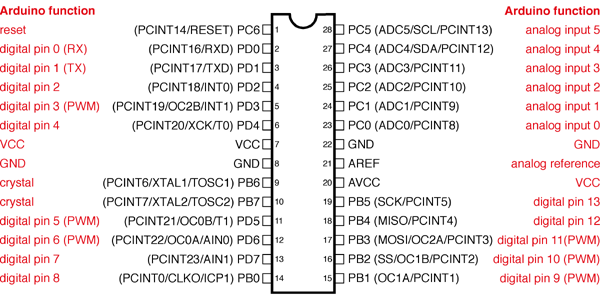
\includegraphics[scale=0.9]{images/atmega328pinout}}
		\caption[ATMega168/328 pinout]{ATMega168/328 pinout (from \protect\parencite{atmega328pinout})}
		\label{fig:atmegapinout}
	\end{figure}
	
\newpage

\section{Custom AVR Board Schematic}\label{app:avrschematic}
	\begin{figure}[H] 
		\centerline{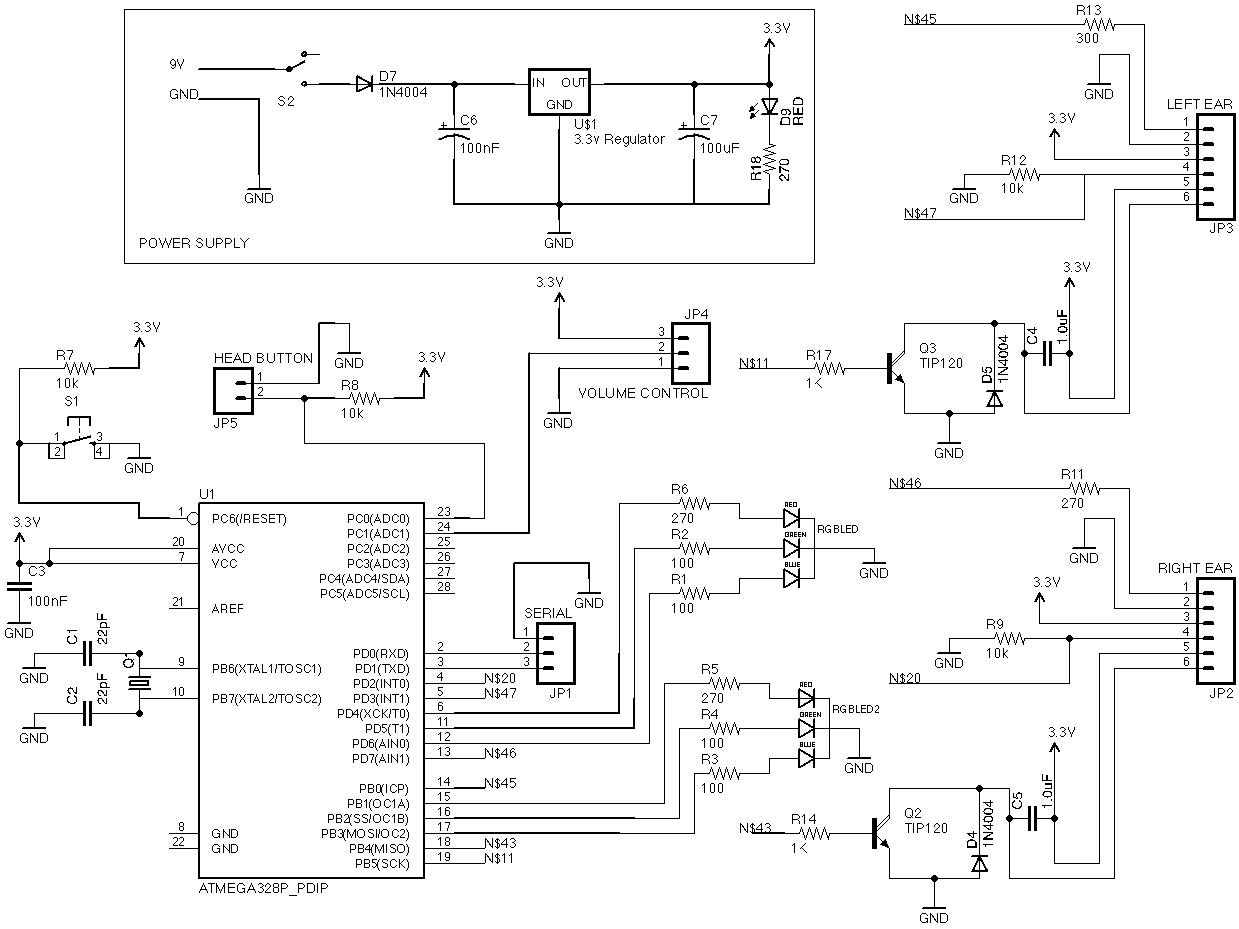
\includegraphics[scale=0.98, angle=90]{images/avrdesign}}
		\caption[Schematic for custom AVR board]{Schematic for custom AVR circuit created to control original \ac{I/O} hardware.}
		\label{fig:avrschematicimage}
	\end{figure}

\newpage
	
\section{Custom AVR Board Prototype}\label{app:prototype}
	\begin{figure}[H] 
		\centerline{\includegraphics[scale=0.2, angle=180]{images/prototype}}
		\caption[Prototype of custom AVR board]{Protoype board created using schematic from Appendix \ref{app:avrschematic}}
		\label{fig:prototypeimage}
	\end{figure}

\newpage
		
\section{Components List}\label{app:componentslist}
	
	\begin{table}[H]
	\centerline{
		\begin{tabular}{ | L{0.22\textwidth} | L{0.07\textwidth} | L{0.3\textwidth} | L{0.28\textwidth} |}
			\hline
			\textbf{Component} & \textbf{Qty.} & \textbf{Function} & \textbf{Source}\\
			\hline
			BeagleBone Black & 1 & Main hardware &  Dr.~Martinez\\
			\hline
			BeagleBone Power Supply & 1 & Main hardware &  Dr.~Martinez\\
			\hline
			USB Wi-Fi Dongle & 1 & Wi-Fi & Dr.~Martinez\\
			\hline
			USB Sound Card & 1 & Sound & Purchased using budget, cost £7.96\\
			\hline
			USB Sound Card & 1 & Sound & Purchased using budget, cost £11.86\\
			\hline
			4 Port USB Hub & 1 & Port expansion & Purchased using budget, cost £4.75\\
			\hline
			2 Port USB Hub & 1 & Port expansion & Purchased using budget, cost £7.10\\
			\hline
			Arduino Duemilanove & 1 & Prototyping & Owned personally\\
			\hline
			ATMega328-PU & 1 & Microcontroller & From Arduino Duemilanove \\
			\hline
			ATMega328-PU & 2 & Microcontroller & Purchased using budget for spares, cost £7.22\\
			\hline
			100nF Capacitor & 1 & Power circuit &  UG Electronics Lab\\
			\hline
			1$\mu$F Capacitor & 2 & Motor circuits &  UG Electronics Lab\\
			\hline
			100$\mu$F Capacitor & 1 & Power circuit &  UG Electronics Lab\\
			\hline
			100$\Omega$ Resistor & 4 & \ac{RGB} \ac{LED}s &  Dr.~Martinez\\
			\hline
			270$\Omega$ Resistor & 7 & \ac{RGB} \& \ac{IR} \ac{LED}s, Ears \& Power Circuit &  Dr.~Martinez\\
			\hline
			1K$\Omega$ Resistor & 2 & Ears &  Dr.~Martinez\\
			\hline
			10K$\Omega$ Resistor & 4 & Ears \& Switches &  Dr.~Martinez\\
			\hline
			\ac{RGB} \ac{LED} & 2 & \ac{LED}s &  Dr.~Martinez\\
			\hline
			Red \ac{LED} & 1 & Power circuit &  Dr.~Martinez\\
			\hline
			3.3v Regulator & 1 & Power  circuit & Dr.~Martinez\\
			\hline
			BC547 NPN Transistor & 2 & Motor circuits & UG Electronics Lab\\
			\hline
			1N4004 Diode & 3 & Power \& motor circuits & UG Electronics Lab\\
			\hline
			Momentary Switch & 1 & AVR Reset & Dr.~Martinez\\
			\hline
		\end{tabular}}
		\caption[Breakdown of components required for project]{Breakdown of components required for project. Total budget use: £38.89}\label{tab:partslist}
	\end{table}
	
\newpage

\section{Serial Communication Protocol Example}\label{app:exampleserial}
	\begin{figure}[H]
		\centering
		\begin{subfigure}{0.95\textwidth}
		\begin{minted}[mathescape,linenos,numbersep=5pt,gobble=3,frame=single, framesep=2mm]{cpp}
			include <SerialCommand.h>
			SerialCommand sCmd;
			
			volatile int leftPinPosition, rightPinPosition;
			
			void setup() {
			  Serial.begin(9600);
			  sCmd.addCommand("EARPOS", EARPOS);
			}
			
			void loop() {
			  sCmd.readSerial();
			}
			
			/*
			EARPOS is called when receiving serial commands of the form
			EARPOS [R|L], it returns the position of the ear over the
			serial port.
			*/
			void EARPOS()
			{
			  char *arg;
			  char earPos;
			  
			  arg = sCmd.next();
			  if (arg != NULL) {
			    earPos = *arg;
			  }
			  
			  switch(earPos){
			    case "R":
			      Serial.println(rightPinPosition);
			      break;
			    case "L":
			      Serial.println(leftPinPosition);
			      break;
			  }
			}
		\end{minted}
		\end{subfigure}
	\caption[Example of Arduino serial command protocol]{Code excerpt demonstrating use of the SerialCommand \protect\parencite{serialcommand} serial protocol library.}
	\label{fig:serialcommandcode}
	\end{figure}
	
\newpage

\section{Interrupt Routine Example}\label{app:exampleisr}
	\begin{figure}[H]
		\centering
		\begin{subfigure}{0.95\textwidth}
		\begin{minted}[mathescape,linenos,numbersep=5pt,gobble=3,frame=single, framesep=2mm]{cpp}
			/*
			EARMOV controls movement of an individual ear.
			The correct interrupt for the ear is enabled, and
			variables for correct functioning of the interrupt are set.
			*/
			void EARMOV(char earSide, int targetPosition){
			  int rotaryPin = (targetPosition + 2) % 17;
			  switch(earSide){
			    case LEFT:
			      attachInterrupt(LEFTEAR_INTERRUPT,moveLeftEar,RISING);
			      leftEarTargetPosition = rotaryPin;
			      seenLeftGap = false;
			      leftInterruptTime = millis();
			      digitalWrite(LEFTEAR_MOTOR, HIGH);
			      break;
			      // Repeated case for right ear omitted.
			  }
			}	
			
			/*
			Interrupt routine for setting the position of the left ear.
			This takes into account the reference gap to ensure that the
			pin position remains correct, e.g. 0-17 (inclusive)
			*/
			void moveLeftEar(){
			  leftPinPosition++;
			  leftLastInterruptTime = leftInterruptTime;
			  leftInterruptTime = millis();
			  leftPulseWidth = leftInterruptTime - leftLastInterruptTime;
			
			  if(leftPulseWidth > 500){
			    leftPinPosition = 0;
			  }
			
			  if(leftPinPosition == leftEarTargetPosition){
			    digitalWrite(LEFTEAR_MOTOR, LOW);
			    sendEarPosition(LEFT, leftPinPosition);
			    attachInterrupt(LEFTEAR_INTERRUPT, leftEarMoved, RISING); 
			  }
			}
		\end{minted}
		\end{subfigure}
		\caption[Example of Arduino ISR code]{Code excerpt demonstrating use of interrupts to change ear position.}
		\label{fig:isrcode}
	\end{figure}

\newpage

\section{Assembled Nabaztag:tag}\label{app:assembled}
	\begin{figure}[H]
		\centerline{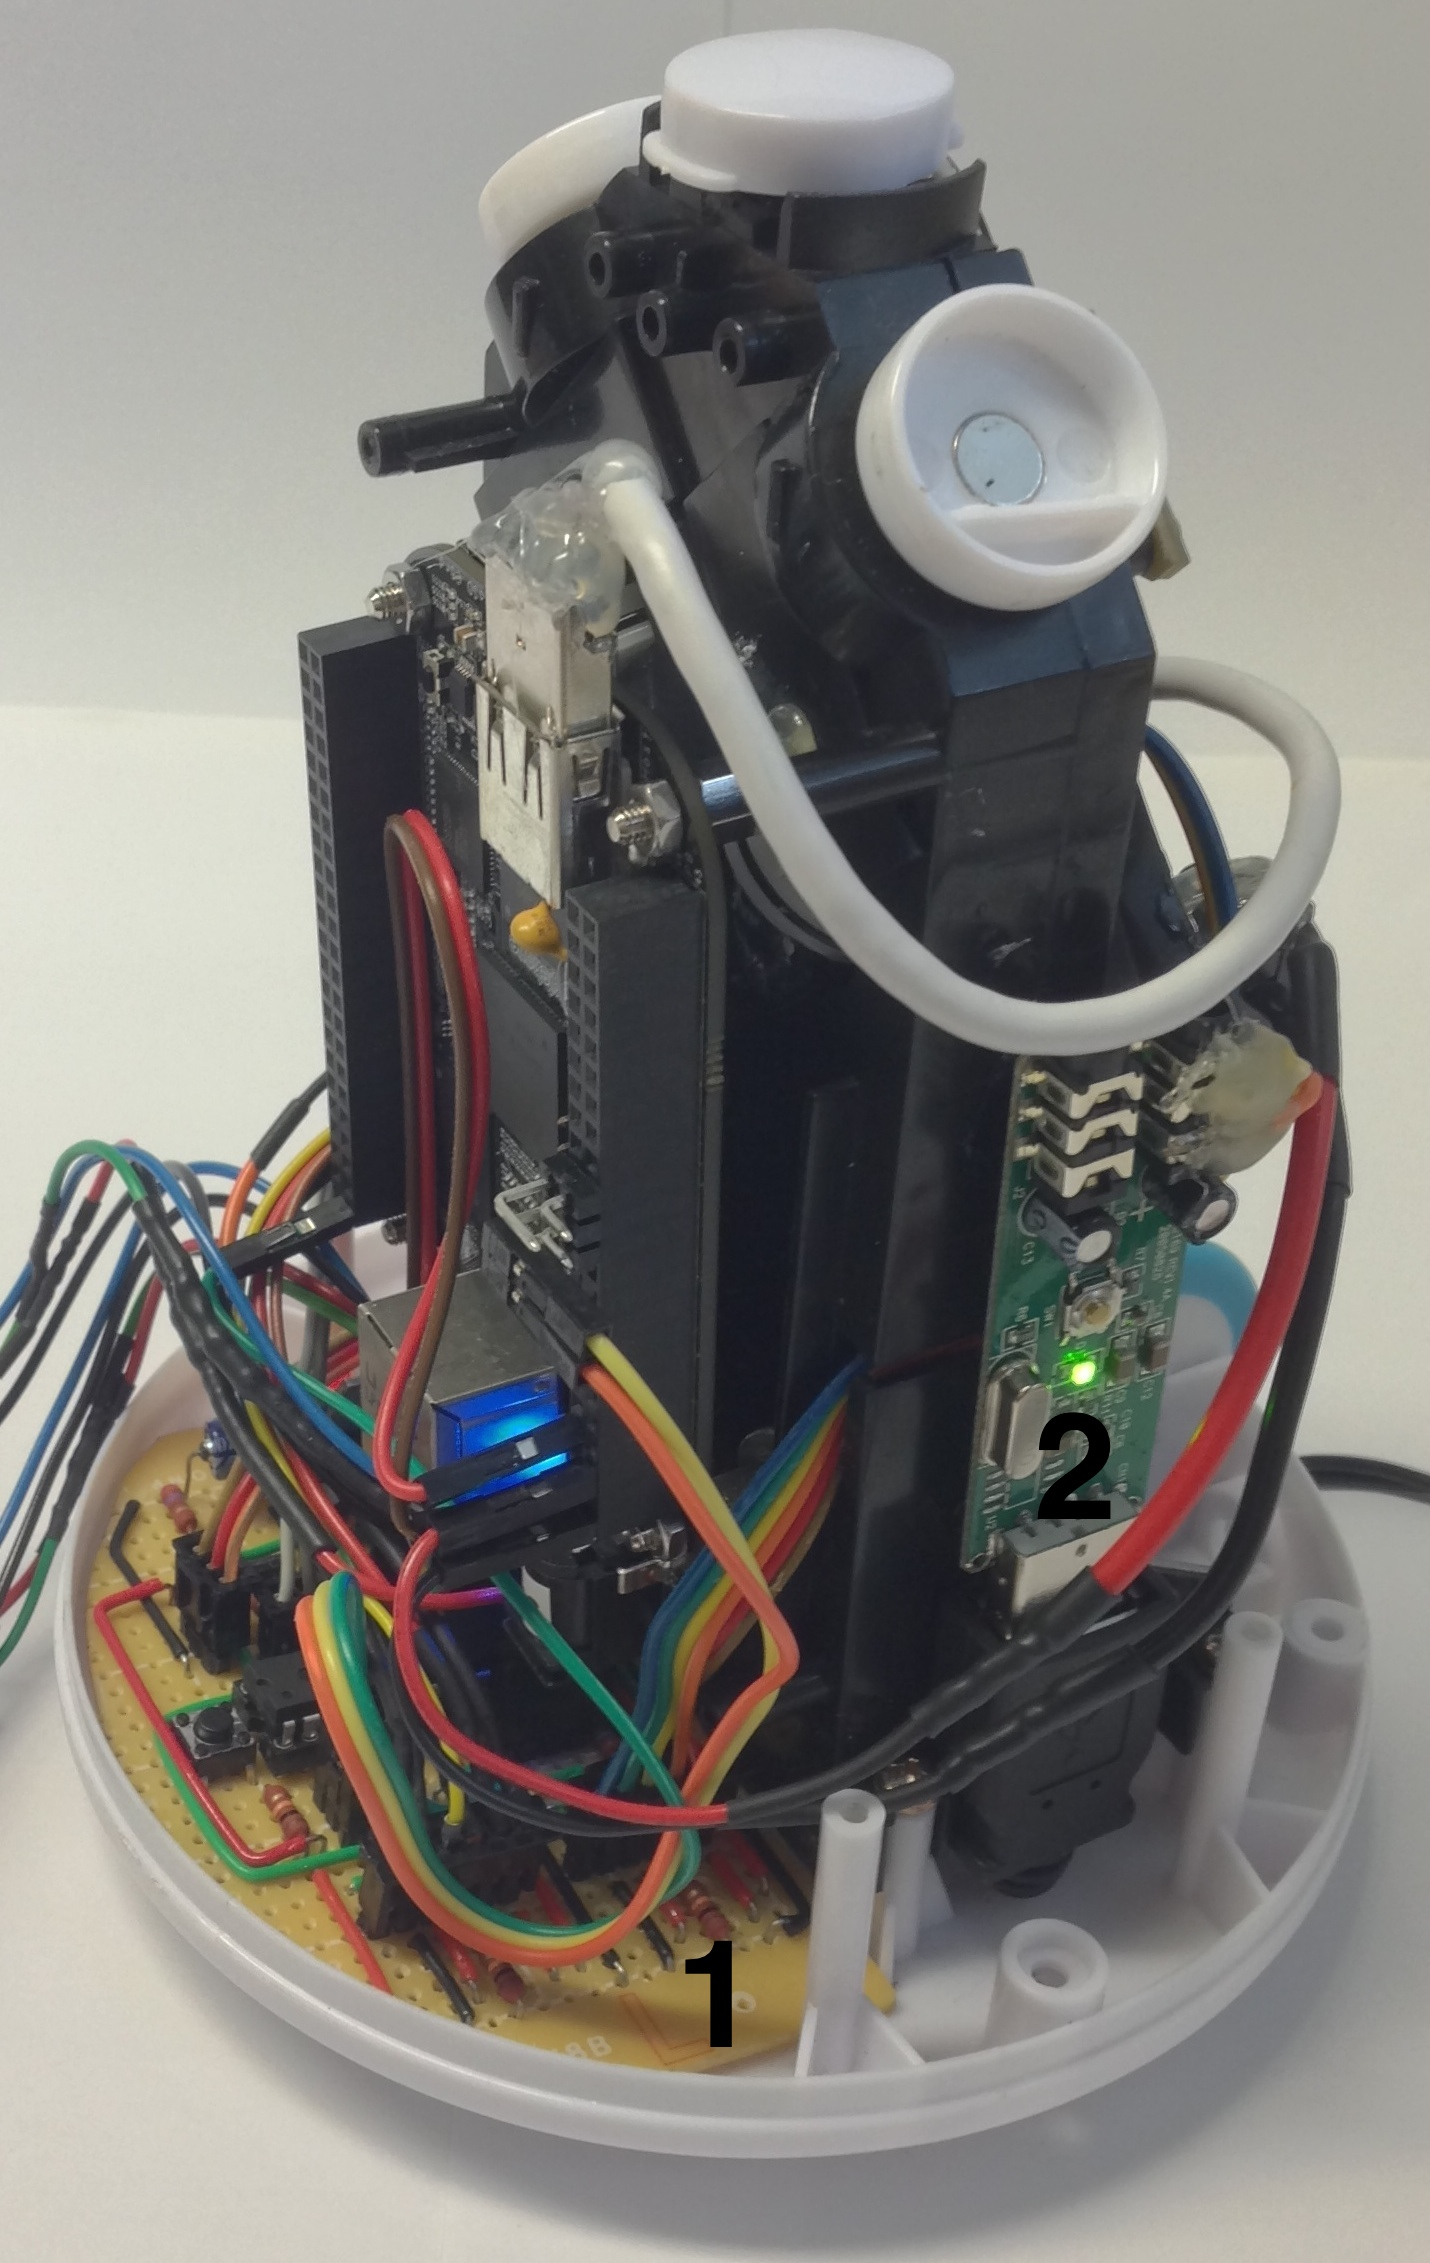
\includegraphics[scale=0.25]{images/nabazleft.jpg}}
		\caption[Assembled Nabaztag:tag 1]{The final assembled form of the Nabaztag:tag replacement hardware. 1) Custom AVR circuit board, 2) \ac{USB} sound card.}
		\label{fig:assembled1}
	\end{figure}
	
	\newpage
	
	\begin{figure}[H]
		\centerline{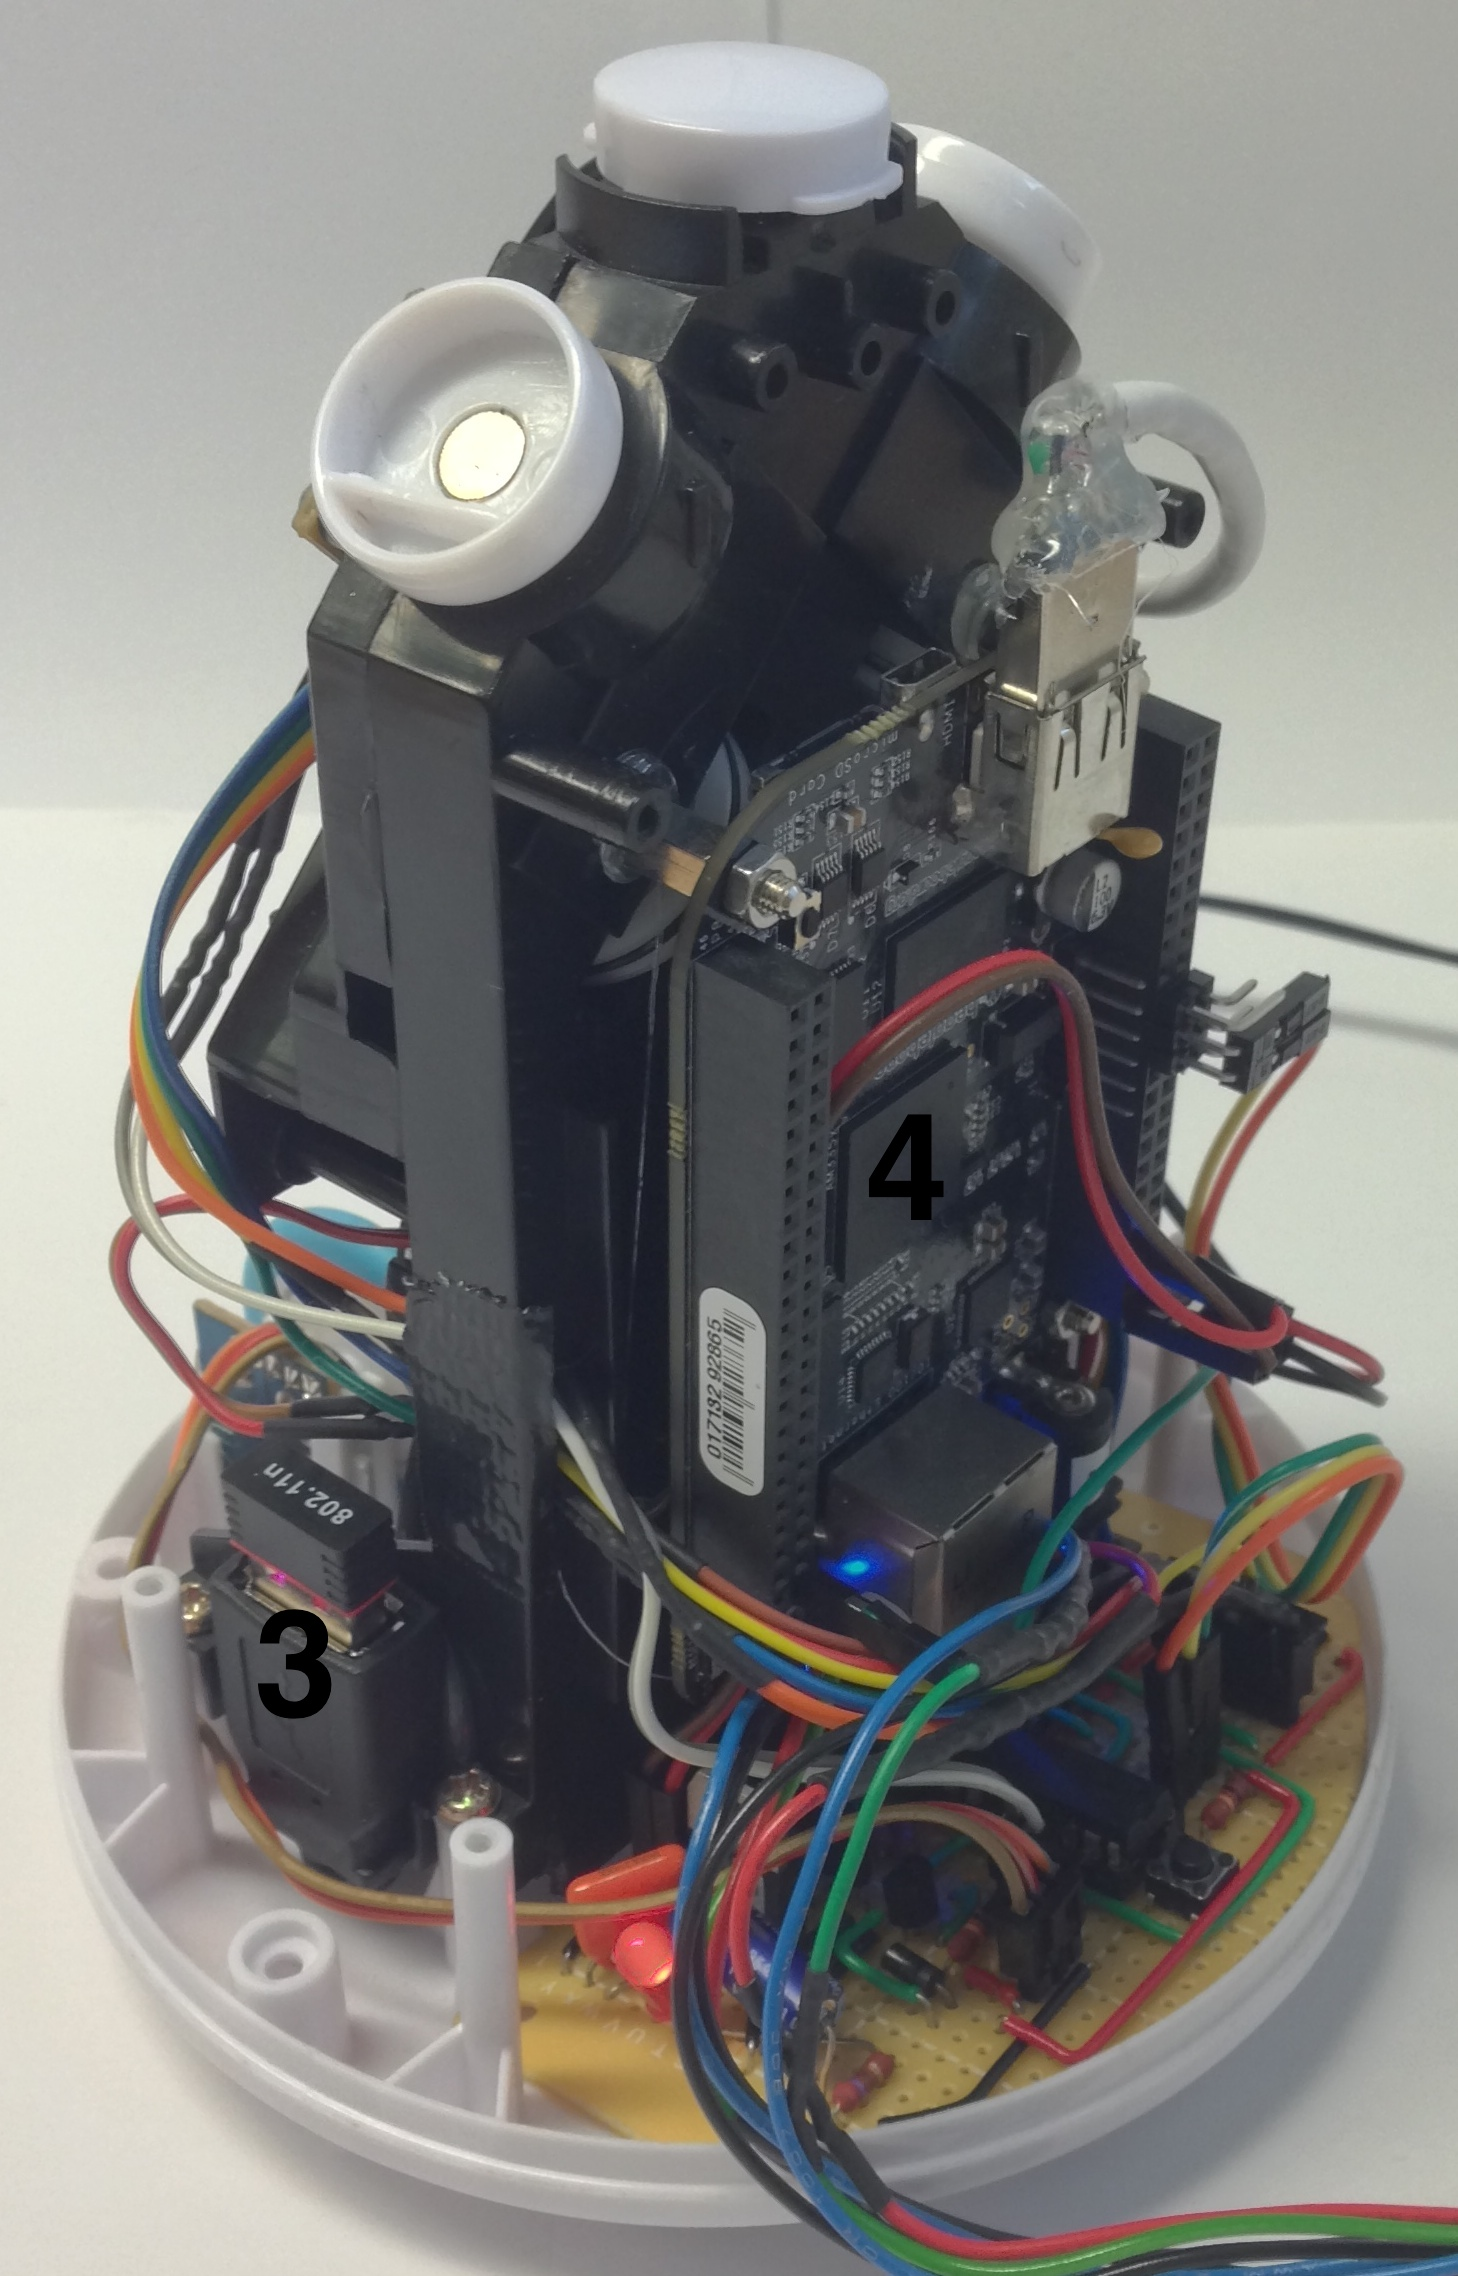
\includegraphics[scale=0.25]{images/nabazright.jpg}}
		\caption[Assembled Nabaztag:tag 2]{The final assembled form of the Nabaztag:tag replacement hardware. 3) \ac{USB} Wi-Fi adapter, 4) \acl{BBB}.}
		\label{fig:assembled2}
	\end{figure}
	
	
\newpage

\section{Web Application Control Page}\label{app:djangoapp}
	\begin{figure}[H]
		\centerline{\includegraphics[scale=0.40]{images/controlpage.png}}
		\caption[Nabaztag:tag web application --- Control page]{An example of the information and control page for a Nabaztag:tag}
		\label{fig:djangoapp}
	\end{figure}
	
\newpage	
	
\section{Sample \acs{API} documentation}\label{app:apidoc}
	\begin{figure}[H] 
		\centerline{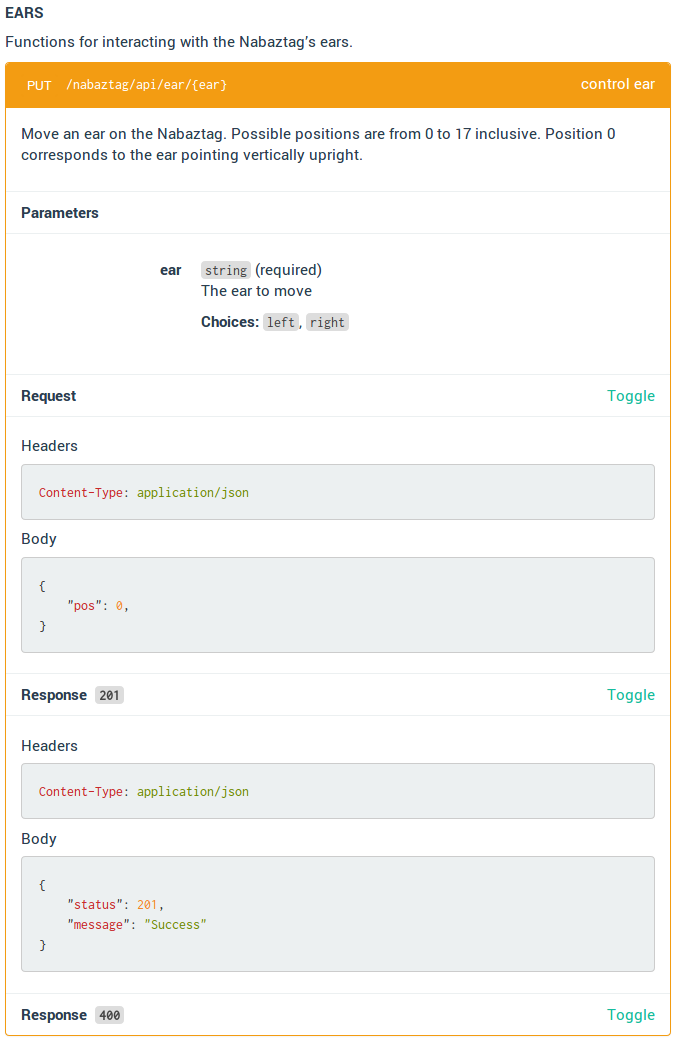
\includegraphics[scale=0.55]{images/apidoc.png}}
		\caption[Example of documentation page for Nabaztag:tag \acs{REST} \acs{API}]{An example of the \ac{API} documentation available from the root of the Nabaztag:tag's \ac{API}}
		\label{fig:apidoc}
	\end{figure}

\newpage
	
\section{Unit Test Results}\label{app:unittests}
	\begin{figure}[H] 
		\centerline{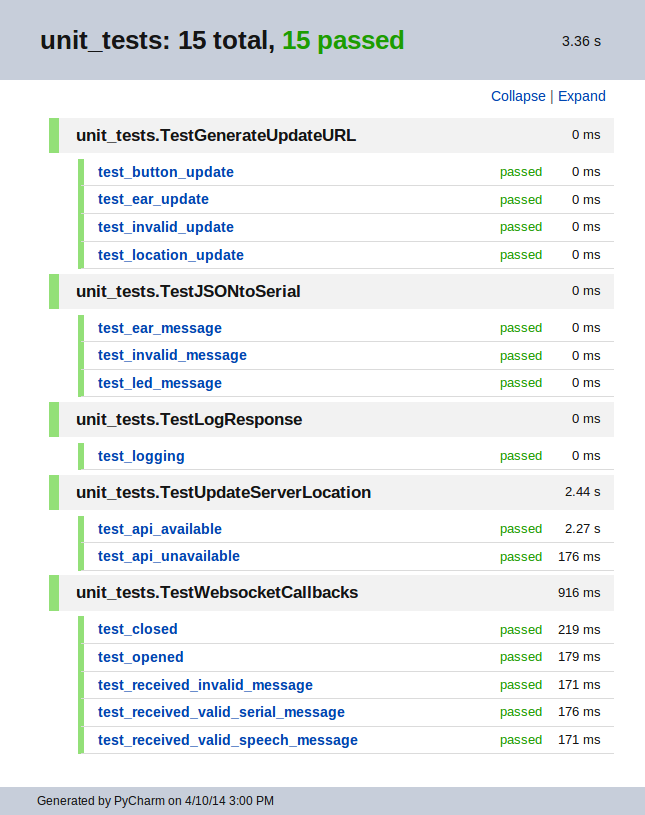
\includegraphics[scale=0.60]{images/unittests.png}}
		\caption[Unit test results for Nabaztag:tag client application]{Unit test results for Nabaztag:tag client application}
		\label{fig:unittests}
	\end{figure}

\newpage

\section{Initial Gantt Charts}\label{app:initialgantt}

	\hvFloat[
	 floatPos=!htb,
	 capWidth=h,
	 capPos=r,
	 capAngle=90,
	 objectAngle=90,
	 capVPos=c,
	 objectPos=c
	]
	{figure}
	{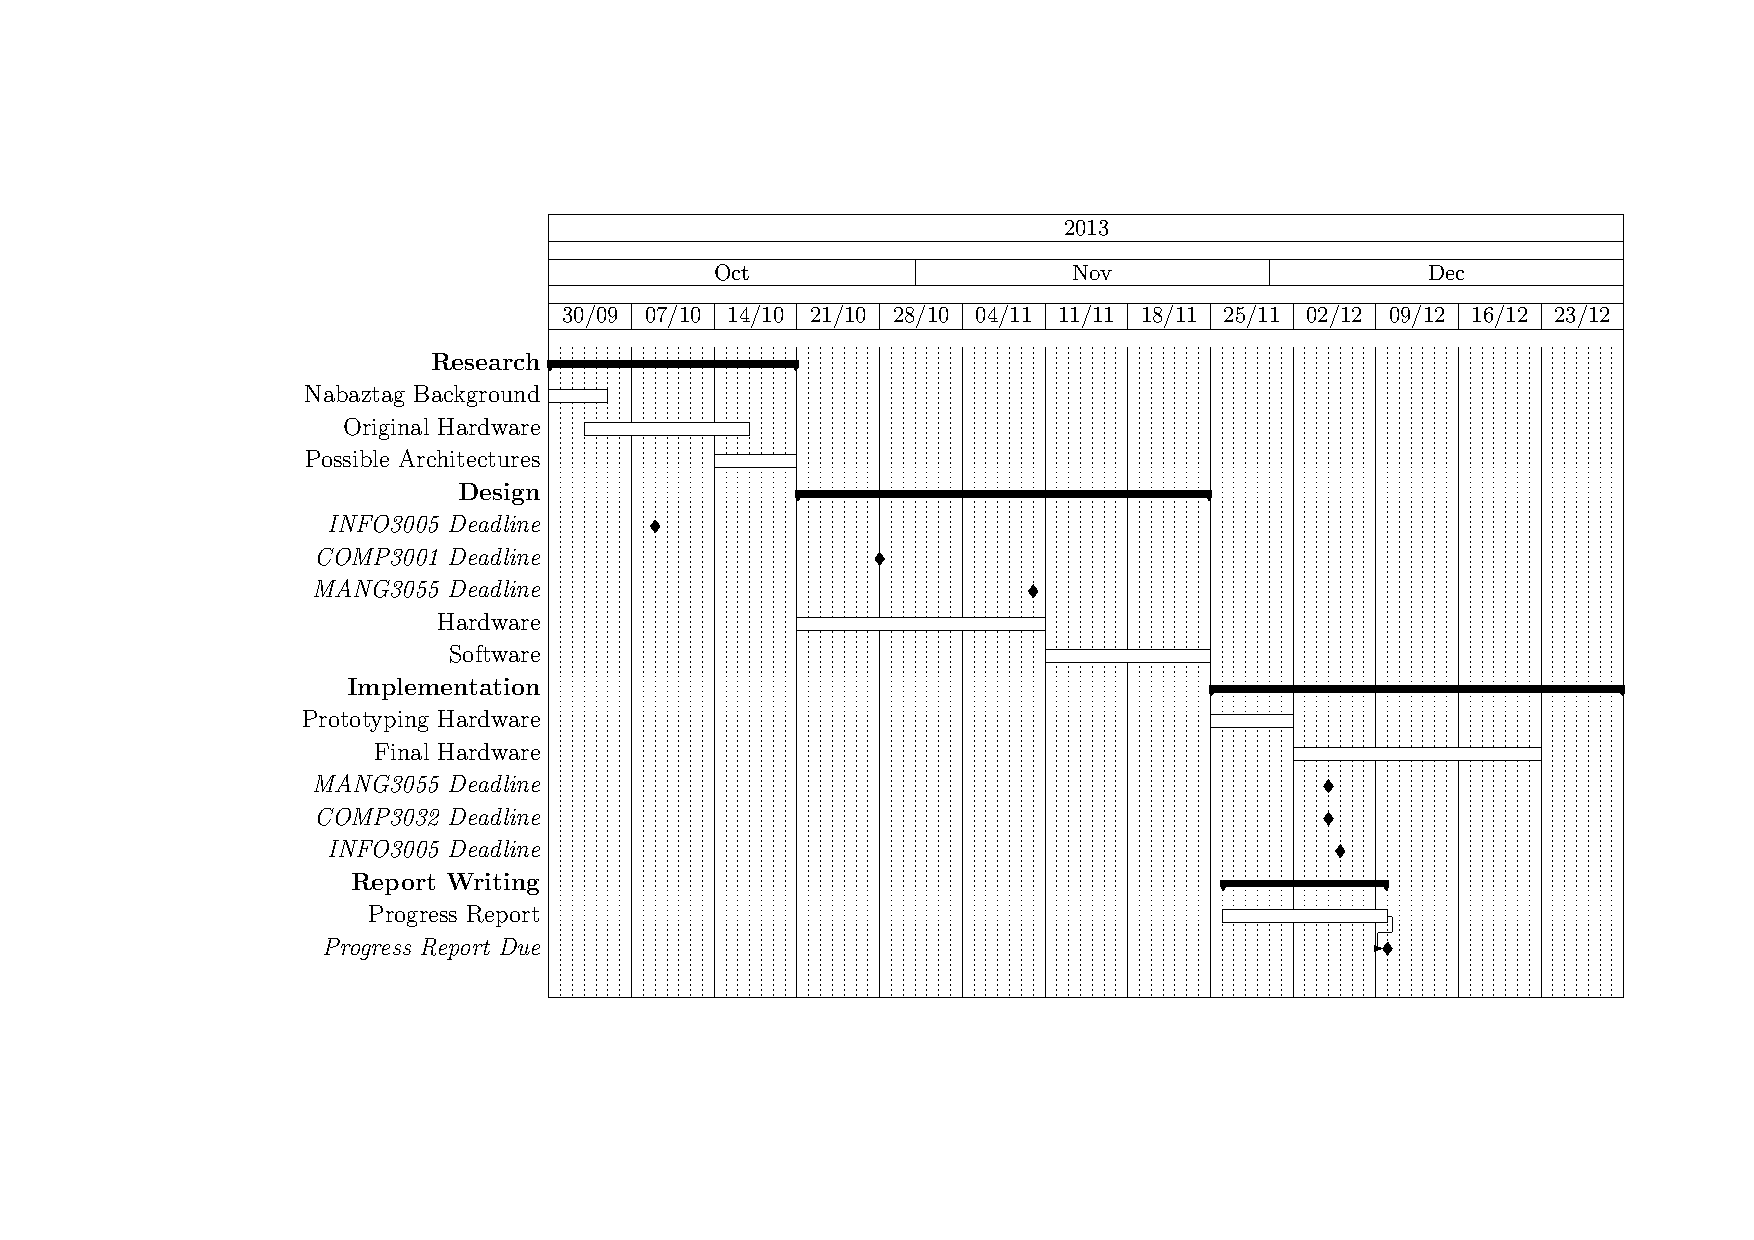
\includegraphics[scale=0.96]{images/origganttone}}
	{Original Semester 1 Gantt chart}
	{fig:ganttone}

	\hvFloat[
	 floatPos=!htb,
	 capWidth=h,
	 capPos=r,
	 capAngle=90,
	 objectAngle=90,
	 capVPos=c,
	 objectPos=c
	]
	{figure}
	{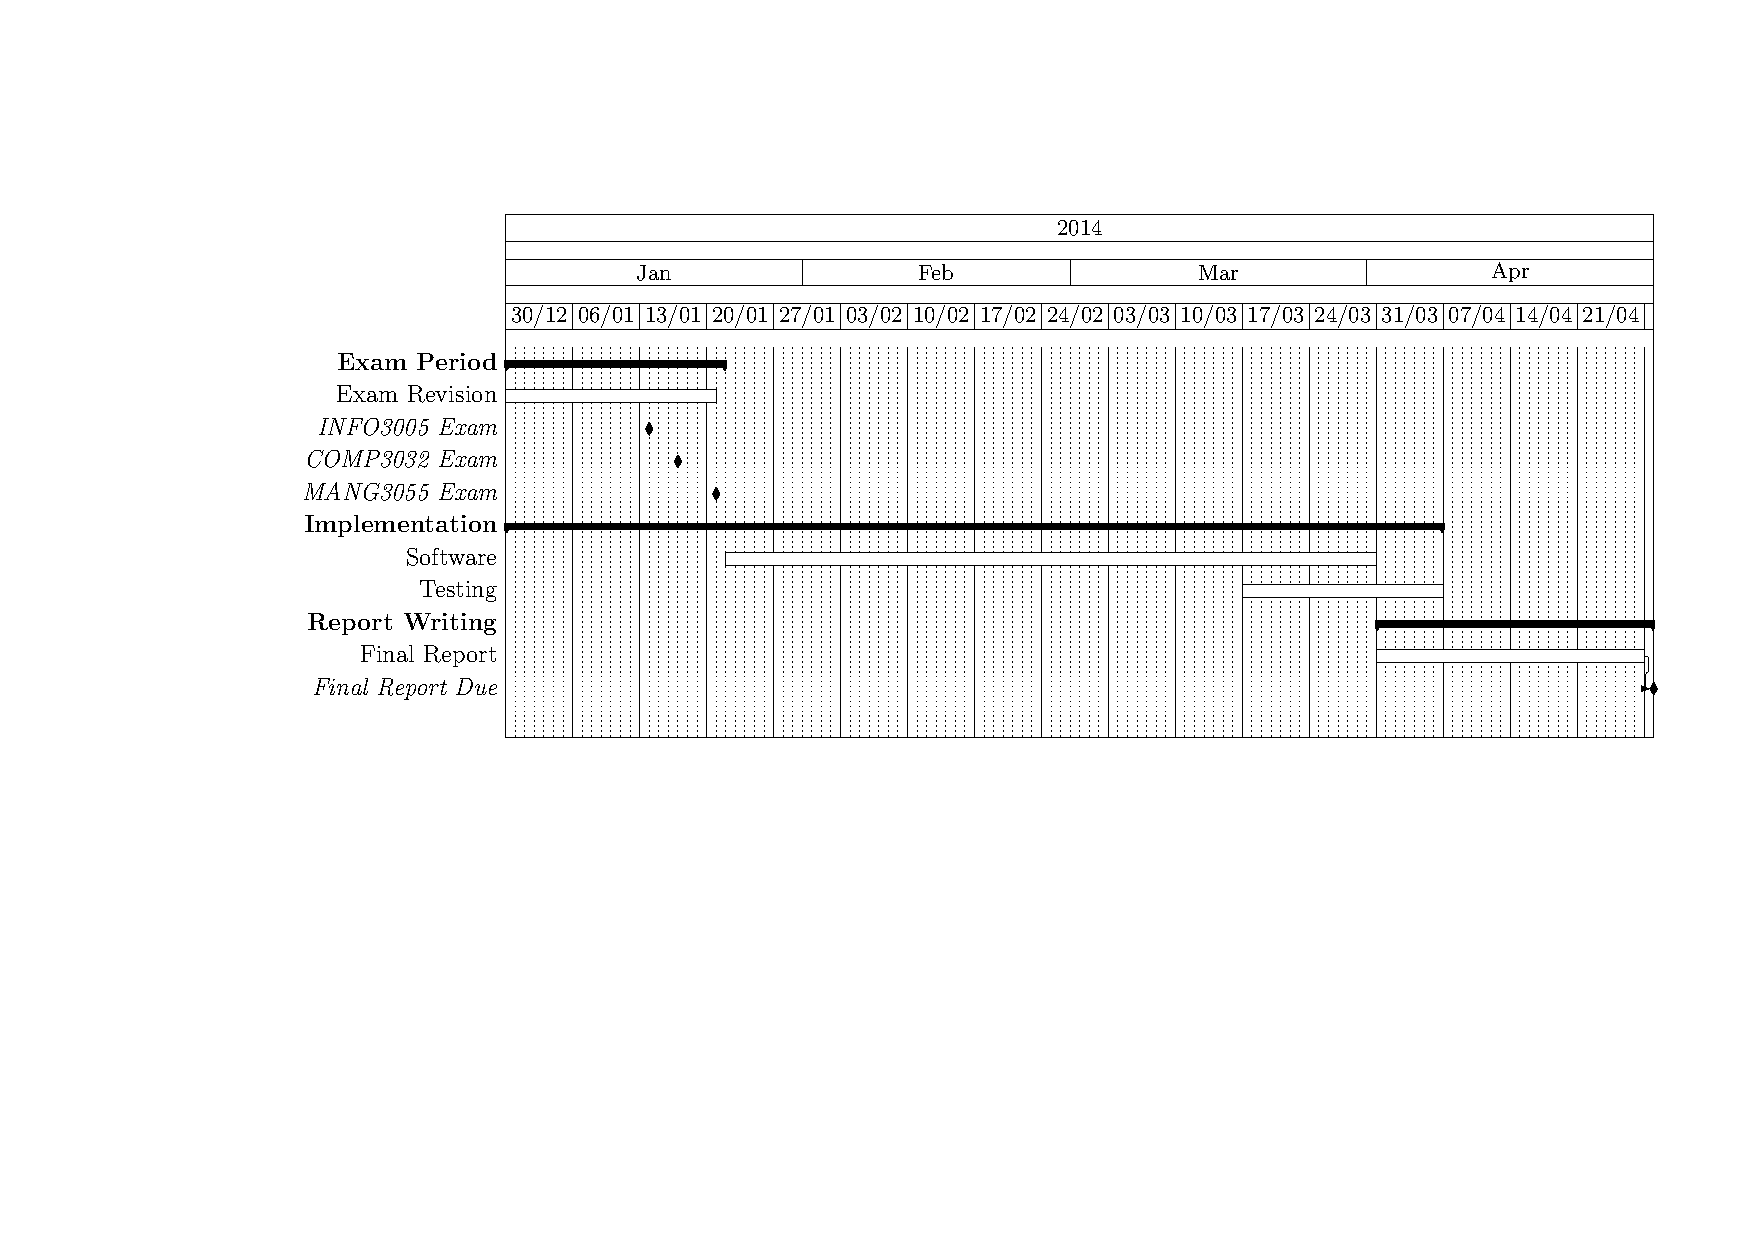
\includegraphics[scale=1]{images/origgantttwo}}
	{Original Semester 2 Gantt chart}
	{fig:gantttwo}
	
\cleardoublepage

\section{Design Archive Listing}\label{app:filelisting}

\begin{figure}[H]
\begin{subfigure}{0.49\textwidth}
\dirtree{%
.1 avr\_setup. 
.2 boards.txt.  
.2 nabaztag\_avr.ino. 
}
\vspace{15pt}
\dirtree{%
.1 beaglebone\_setup. 
.2 BB-UART1.dts. 
.2 LED\_blink\_test.py. 
.2 LED\_fade\_test.py. 
.2 README.md. 
.2 dtc\_patcher.sh.
}
\vspace{15pt}
\dirtree{%
.1 nabaztagclient. 
.2 beaglebone. 
.3 \_\_init\_\_.py. 
.3 nabaztag\_client.py. 
.3 nabaztag\_serial.py. 
.3 nabaztag\_update.py. 
.3 nabaztag\_upstart.conf. 
.3 nabaztag\_websocket.py. 
.2 nabaztagconfig.yaml. 
.2 pi. 
.3 pi\_button.py. 
.3 pi\_client.py. 
.3 pi\_update.py. 
.3 pi\_upstart.conf. 
.3 pi\_websocket.py. 
.2 restapi. 
.3 documentation. 
.4 nabaztagapi\_blueprint.md. 
.4 nabaztatgapi\_static.html. 
.3 nabaztagapi\_geolocate.py. 
.3 nabaztagapi\_nginx.conf. 
.3 nabaztagapi\_server.py. 
.3 nabaztagapi\_upstart.conf. 
.3 nabaztagapi\_weather.py. 
.2 unit\_tests.py.
}
\end{subfigure}
~~~
\begin{subfigure}{0.49\textwidth}
\dirtree{%
.1 nabaztagserver. 
.2 deployment. 
.3 README.md. 
.3 django\_uwsgi.ini. 
.3 nginx.conf. 
.3 uwsgi.conf. 
.3 uwsgi\_params. 
.3 websocket\_uwsgi.ini. 
.2 manage.py. 
.2 nabaztag. 
.3 \_\_init\_\_.py. 
.3 admin.py. 
.3 forms.py. 
.3 models.py. 
.3 templates.
.4 control.html. 
.4 index.html. 
.3 urls.py. 
.3 views.py. 
.2 nabaztagserver. 
.3 \_\_init\_\_.py. 
.3 settings.py. 
.3 urls.py. 
.3 wsgi\_django.py. 
.3 wsgi\_websocket.py. 
}
\end{subfigure}
\caption{Directory listing for project files included in Design Archive}
\label{fig:filelist}
\end{figure}

\newpage
	
\section{Original Project Brief}\label{app:originalbrief}

	\textbf{This was the initial brief submitted for the project, it is included for reference:}
	
	The Nabaztag, developed by Violet and first released in 
	2005, was an attempt at introducing pervasive computing to the masses. 
	A wi-fi enabled smart device, shaped to look like a rabbit, with a 
	variety of functions. Nabaztag could convey information through 5 
	multicoloured LEDs, motorised ears, and built-in speaker, and could 
	receive input from its environment using a push button, a microphone, 
	an RFID reader and by manual adjustment of the position of its ears.
	
	Nabaztag relied heavily on communication with servers 
	operated by Violet, which stored the majority of its configuration 
	information, and provided the only way for a Nabaztag owner to alter 
	the behaviour of their device. In December 2006, when large numbers of 
	purchased Nabaztag devices were activated simultaneously, Violet's 
	infrastructure was unable to cope with the demand, and there were 
	service disruptions for both new and existing Nabaztag owners. In 
	October 2009, after a long period of technical troubles, Violet 
	declared bankruptcy and was purchased by an Australian software house, 
	Mindscape. In July 2011, Mindscape stopped maintaining the Nabaztag, 
	and released the previously closed source code to the public. Efforts 
	to understand the Nabaztag architecture have been hindered by the 
	poor documentation, and by existing documentation being in French.
	
	Several open source projects have attempted to create new web 
	interfaces for the Nabaztag, but they suffer from the requirement that 
	they must interact with the original software running 
	on the proprietary, single-board computer that is at the heart of the 
	Nabaztag. While compatibility with the client software on the Nabaztag is
	necessary to allow existing Nabaztag owners 
	to return functionality to their devices without any complex modifications,
	it limits the potential to experiment with new and improved technologies 
	which might be used to address the original issues with the Nabaztag architecture.
	
	In this project, I intend to bring a single Nabaztag back to 
	life. I wish to as a minimum restore its previous functionality, and 
	potentially add new functionality not present on the original 
	device. To achieve this, broadly I will:
	
	\begin{itemize}
		\item Replace the single-board computer in the Nabaztag with a modern open 
	hardware device such as the BeagleBone Black, whilst maintaining all 
	the original input and output hardware of the Nabaztag.
		\item Develop a client application, able to run on the open 
	hardware device and control all functionality of the Nabaztag,.
		\item Develop a server application, able to communicate with 
	the client application using a push notification architecture.
		\item Develop a web interface to the server application, 
	allowing users to interact with their Nabaztag by pushing updates and configuration changes from 
	server to client.
	\end{itemize}

\end{appendices}	
%TC:endignore

\end{document}
